%%%%%%%%%%%%%%%%%%%%%%%%%%%%%%%%%%%%%%%%%%%%%%%%%%%%%%%%%%%%%%%%%%%%%%%%
%#BIBTEX bibtex esmgw1
%   names Takao Kotani, Hiori Kino Hisazumi Akai
%
% address
%         Department of applied physics and materials, Tottori university,
%
% E-mail  takaokotani@gmail.compvv
%
%%%%%%%%%%%%%%%%%%%%%%%%%%%%%%%%%%%%%%%%%%%%%%%%%%%%%%%%%%%%%%%%%%%%%%%%%
%\documentclass[twocolumn,showpacs,preprintnumbers,amsmath,amssymb,floatfix]{revtex4-1}
\documentclass[twocolumn,superscriptaddress,showpacs,preprintnumbers,amsmath,amssymb,prb]{revtex4-1}
%\documentclass[preprint,superscriptaddress,showpacs,preprintnumbers,amsmath,amssymb,prb]{revtex4-1}

% Some other (several out of many) possibilities
%\documentclass[aps,prl,preprint,groupedaddress,showpacs]{revtex4}
%\documentclass[aps,prl,twocolumn,superscriptaddress,showpacs]{revtex4}
%\documentclass[aps,prb,preprint,superscriptaddress,showpacs]{revtex4}

\usepackage{multirow}
%\usepackage{graphicx}
\usepackage[dvipdfmx]{graphicx, color,hyperref}
\usepackage{pxjahyper}
\usepackage{longtable}
\usepackage{dcolumn}% Align table columns on decimal point
\usepackage{bm}% bold math
%\usepackage{pst-all}      % From PSTricks
\usepackage{fancybox}
\usepackage{lineno}
%\topmargin=.0cm
%\nofiles
\newcommand{\rou}[1]{\noindent------------------------------------------------------------------------------------------------------------
\noindent{\bf \large #1}}
\newcounter{Alist}
\newcommand{\ul}[1]{\underline{#1}}
%%%%%%%%%%%%%%%%%%%%%%%%%%%%%%%%
\newcommand{\ocite}[1]{\cite{#1}}

\newcommand{\ispone}{}
\newcommand{\isptwo}{}
\newcommand{\ooplus}{\oplus}
\newcommand{\oominus}{\ominus}

\newcommand{\parahead}[1]{\textcolor{blue}{#1.--}}
\usepackage{color}
\newcommand{\redtx}[1]{\textcolor{red}{#1:}}

\def\connect#1{\leavevmode{\setbox1=\hbox{#1}\copy1%
\raise .2\ht1 \vbox{\moveleft \wd1\vbox{\hrule width \wd1 height .5pt depth 0pt}}%
}}
%\def\we{\connect{\mbox{$\omega\varepsilon$}}}

%\topmargin =0mm
\special{papersize=8.267 in, 11.692 in}
\bibliographystyle{apsrev4-1}
\linenumbers
%%%%%%%%%%%%%%%%%%%%%%%%%%%%%%%%%%%%%%%%%%%%%%%%%%%%%%%%%%%%%%%%%%%%%%%%%%
\begin{document}
%\special{papersize=8.5 in, 11 in}
\title{Supplement: Comparison of day-by-day reproductivity of COVID-19 among countries
by a newly-developed reproduction index $R^{\rm W9}$}
\author{Takao Kotani}
\email{takaokotani@gmail.com}
\author{Motonari Sawada}
\author{Hirofumi Sakakibara}

\affiliation{Department of Applied Mathematics and Physics, Tottori university, Tottori 680-8552, Japan}


\date{\today}
\maketitle


% --------------- Introduction ------------------


\begin{figure*}[ht]
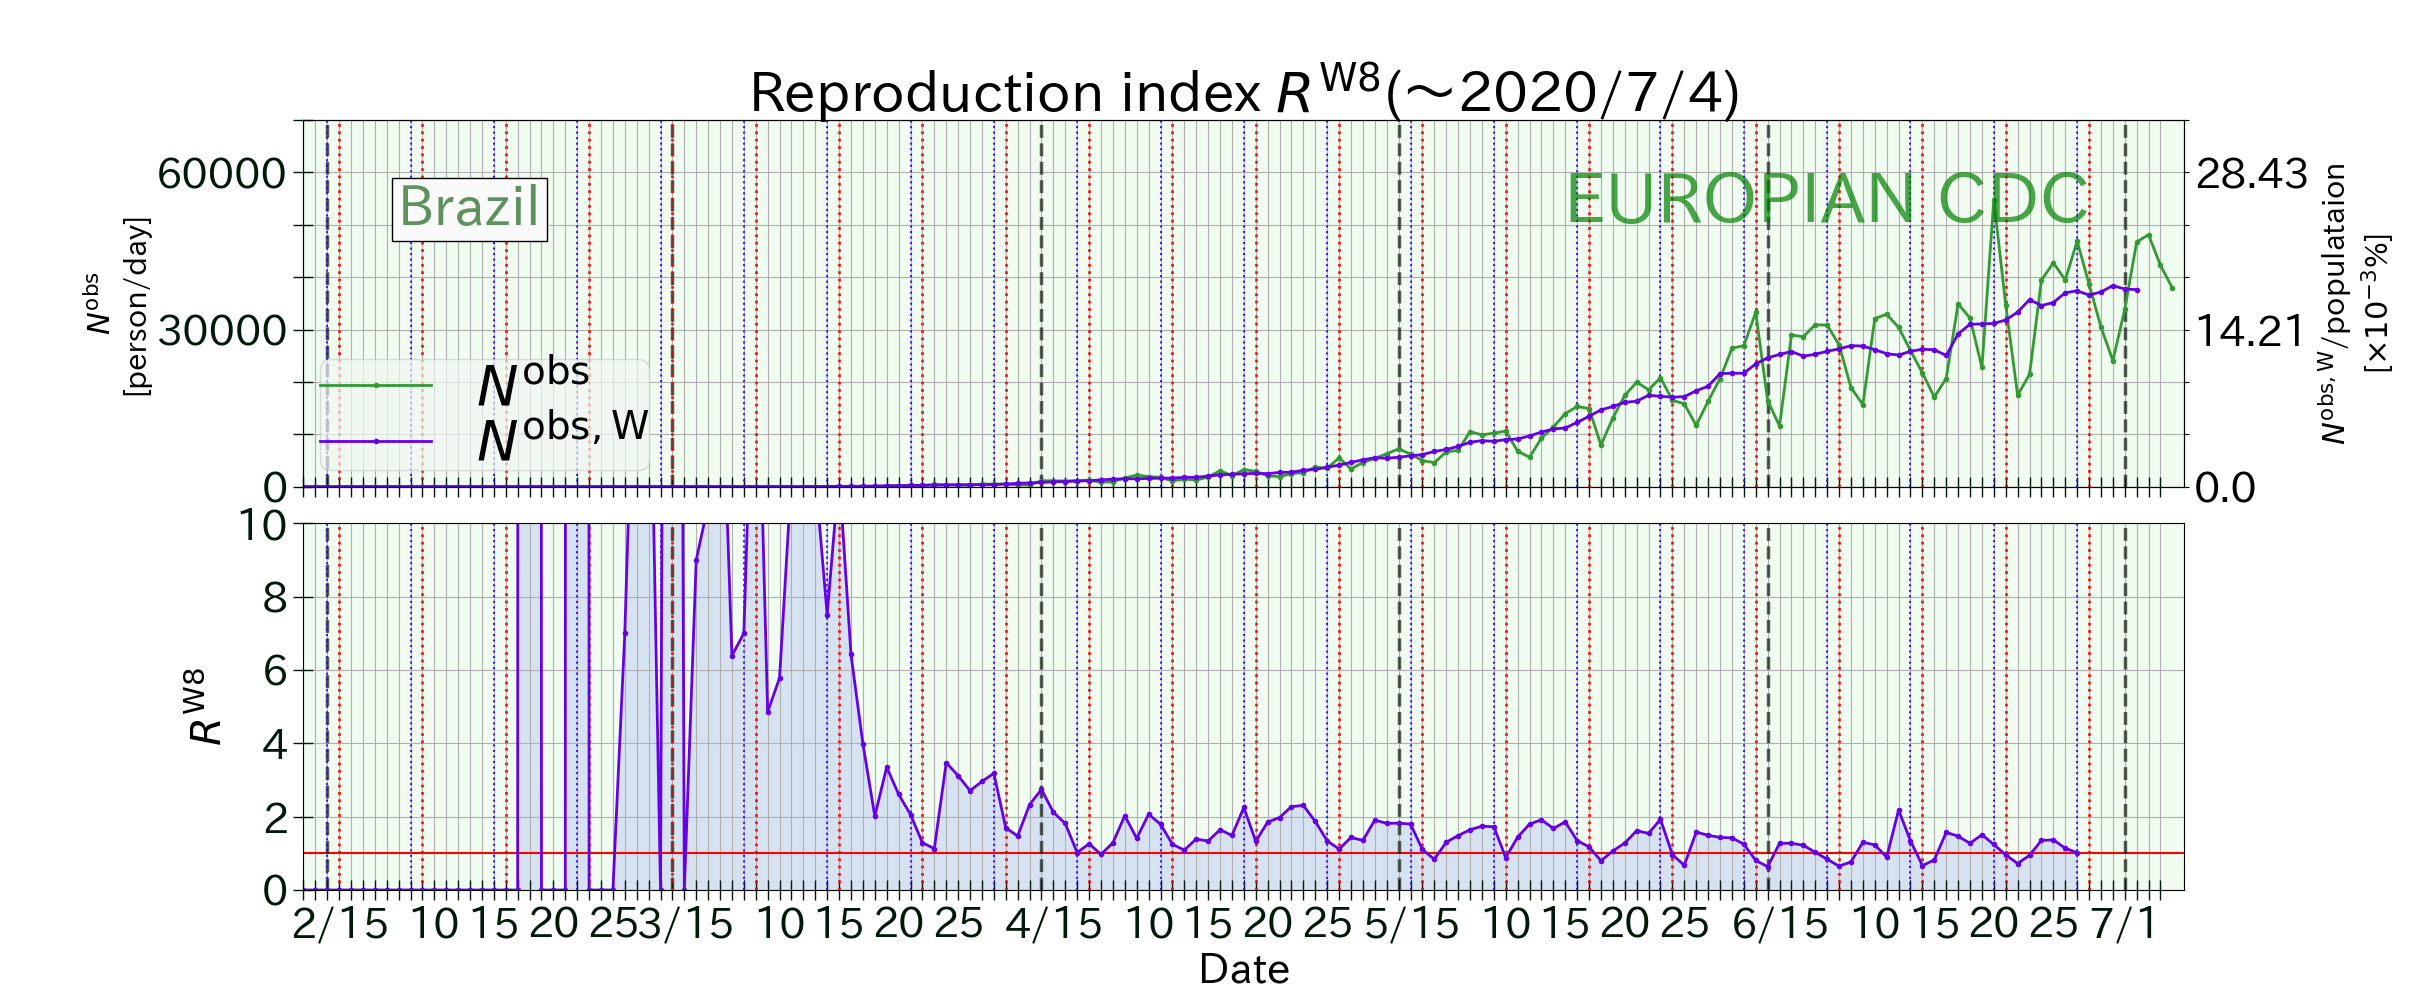
\includegraphics[width=8.9cm]{Brazil.png}
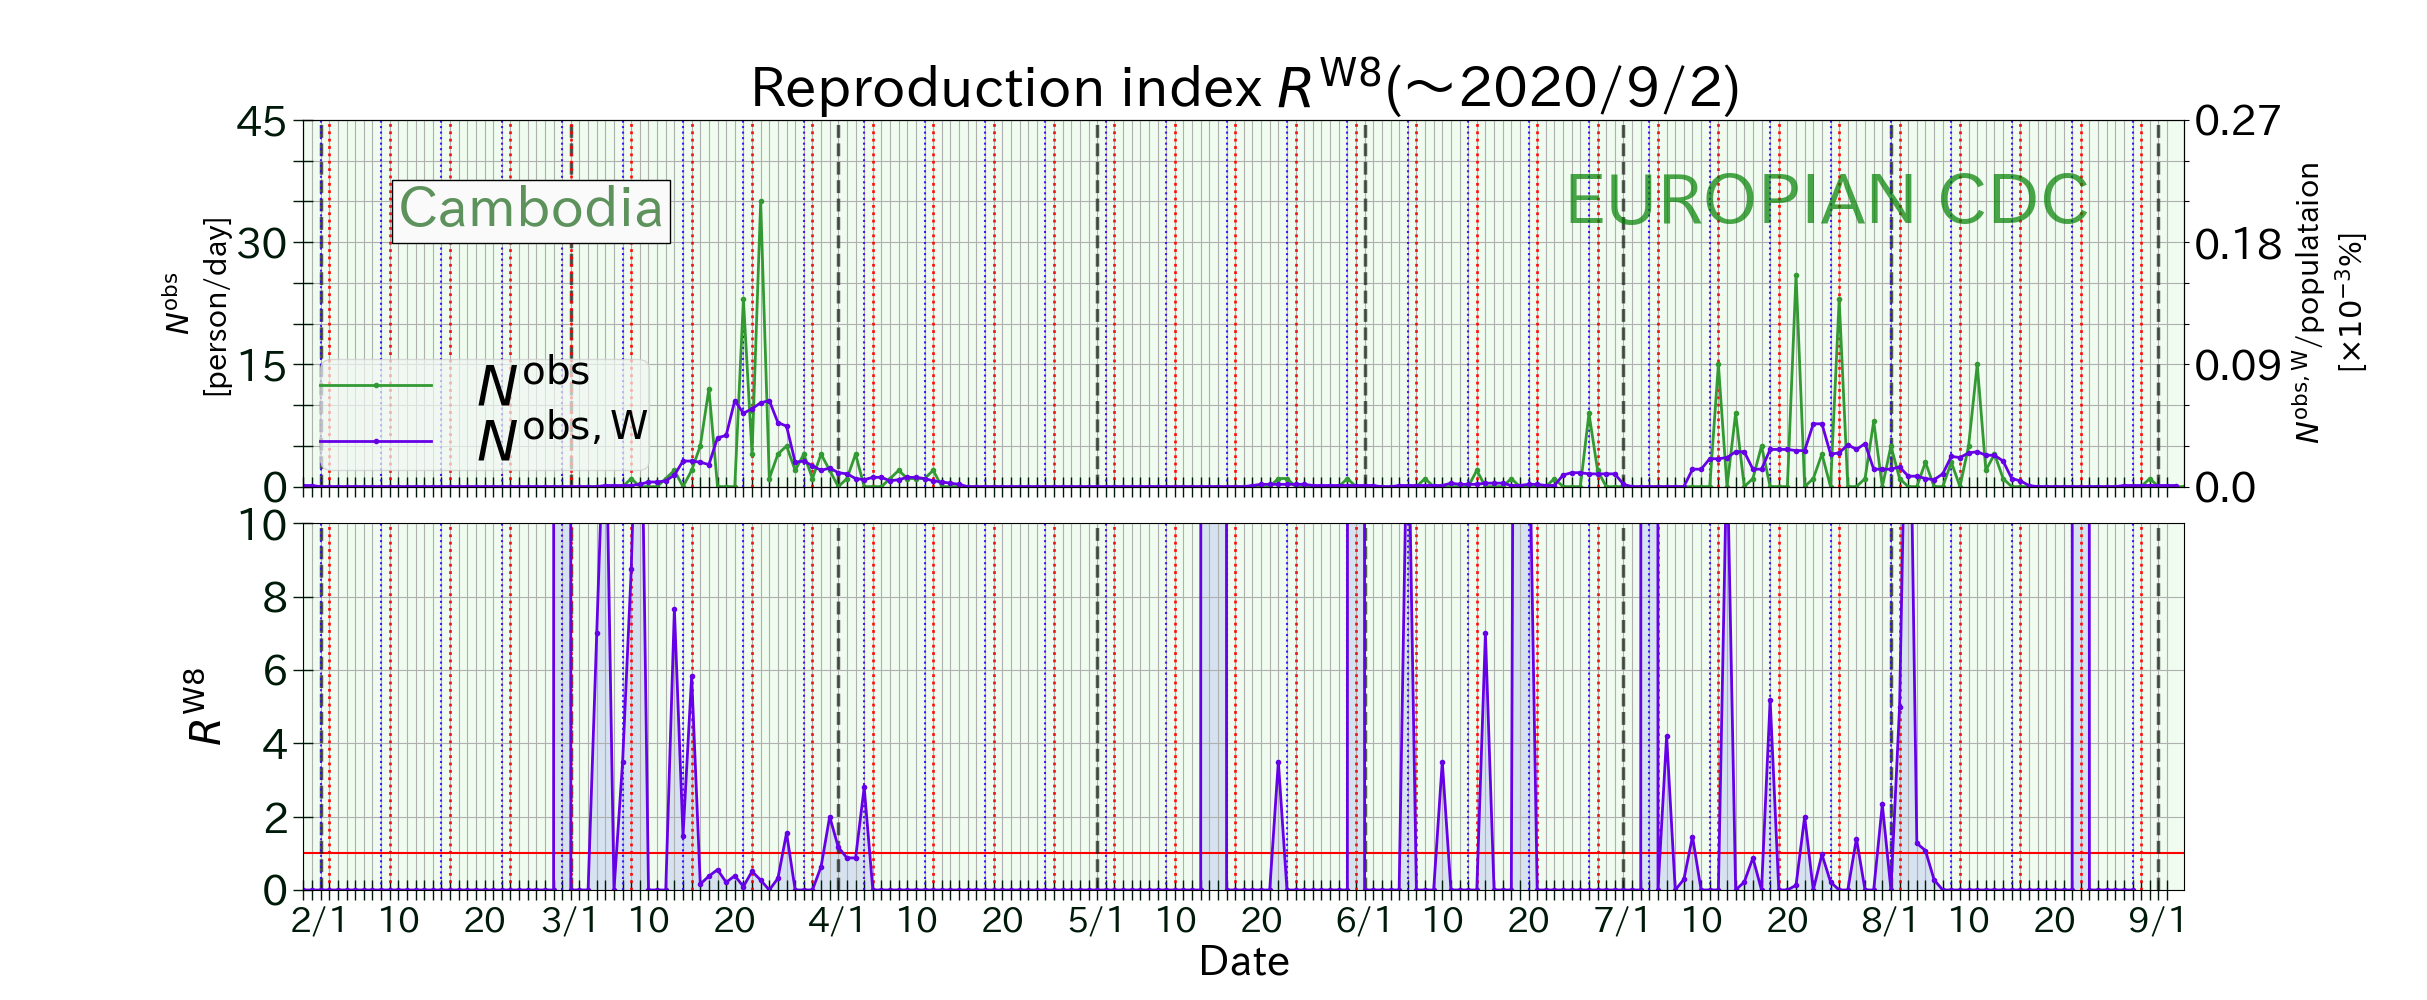
\includegraphics[width=8.9cm]{Cambodia.png}
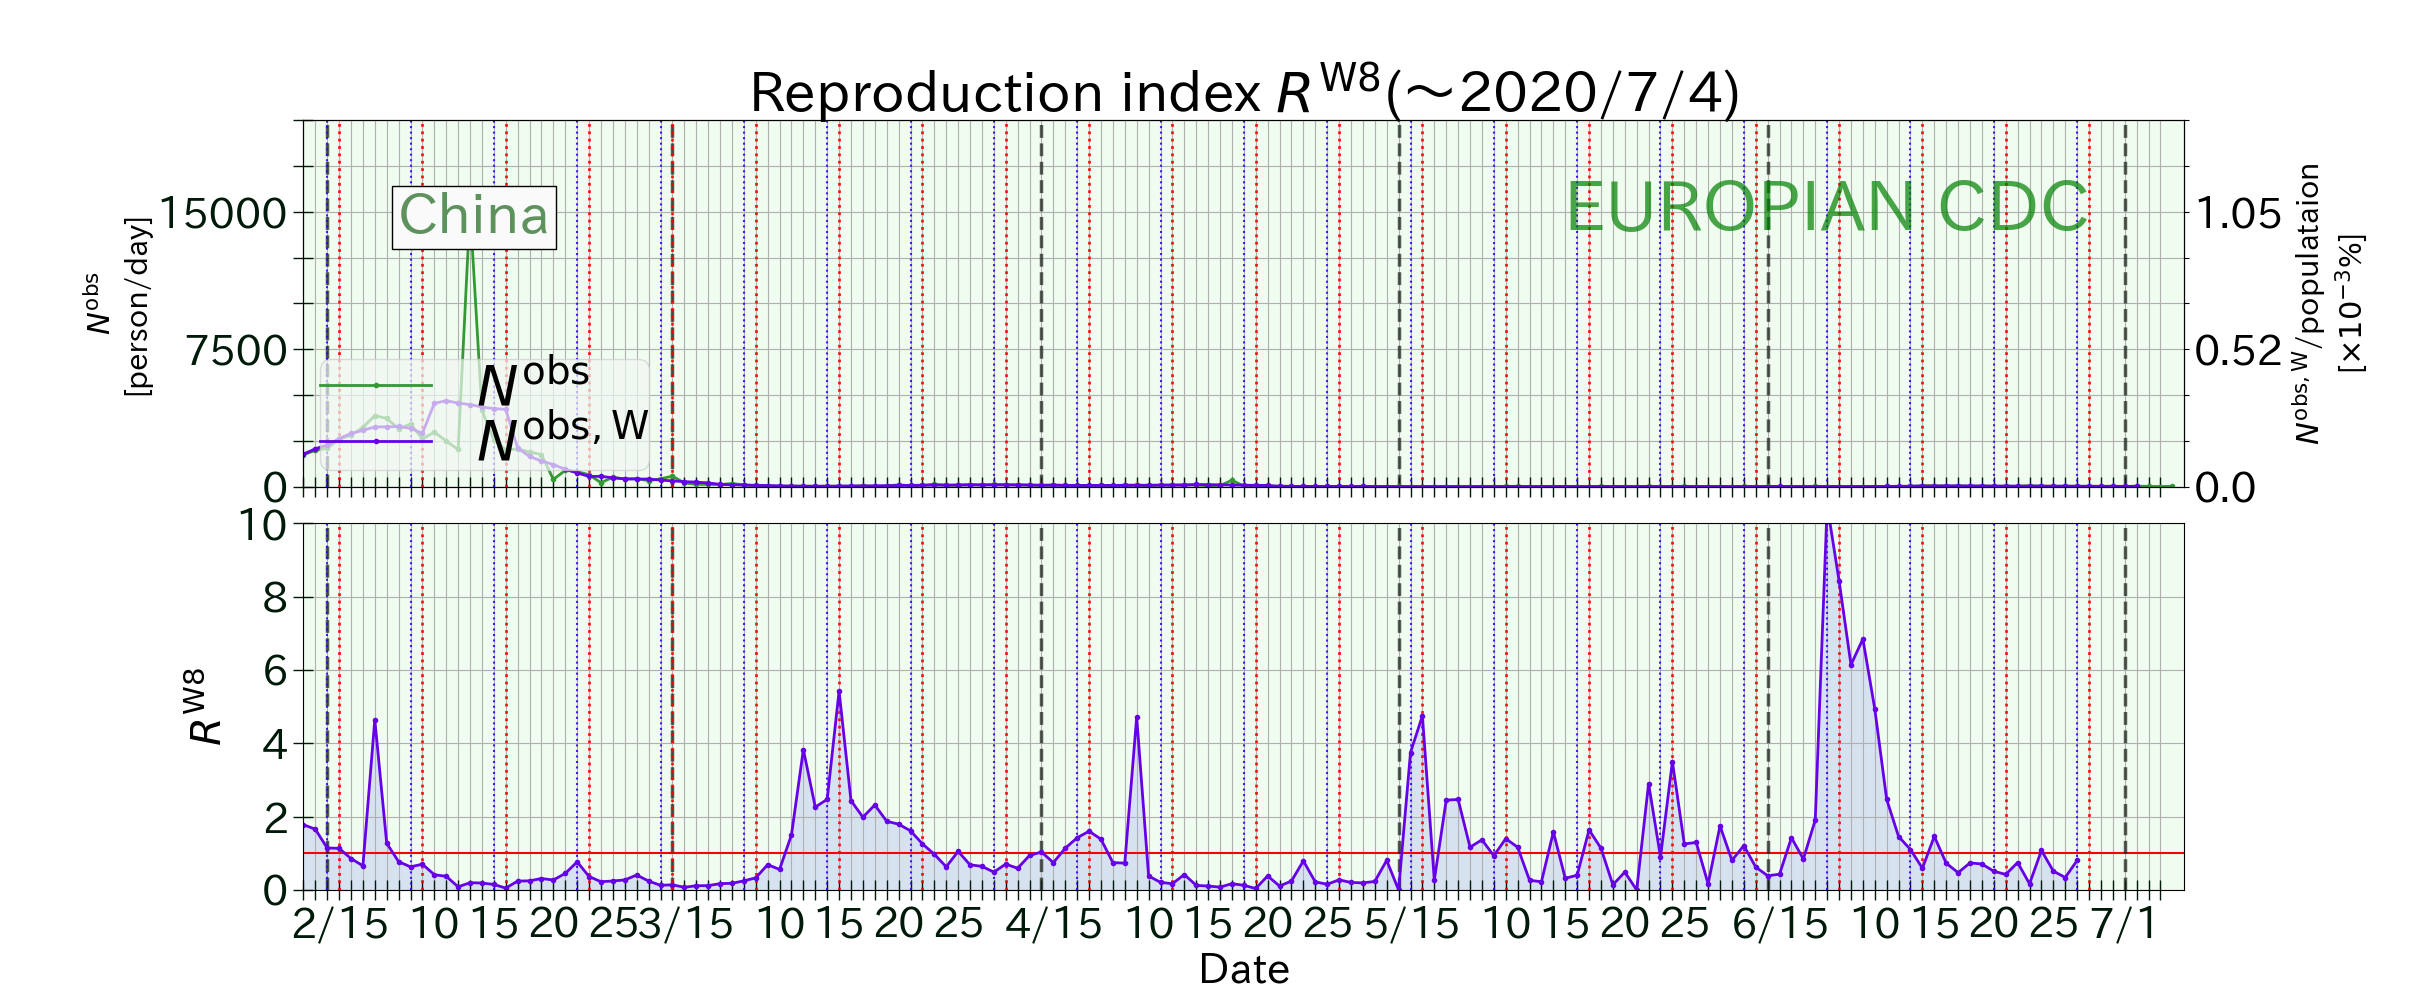
\includegraphics[width=8.9cm]{China.png}
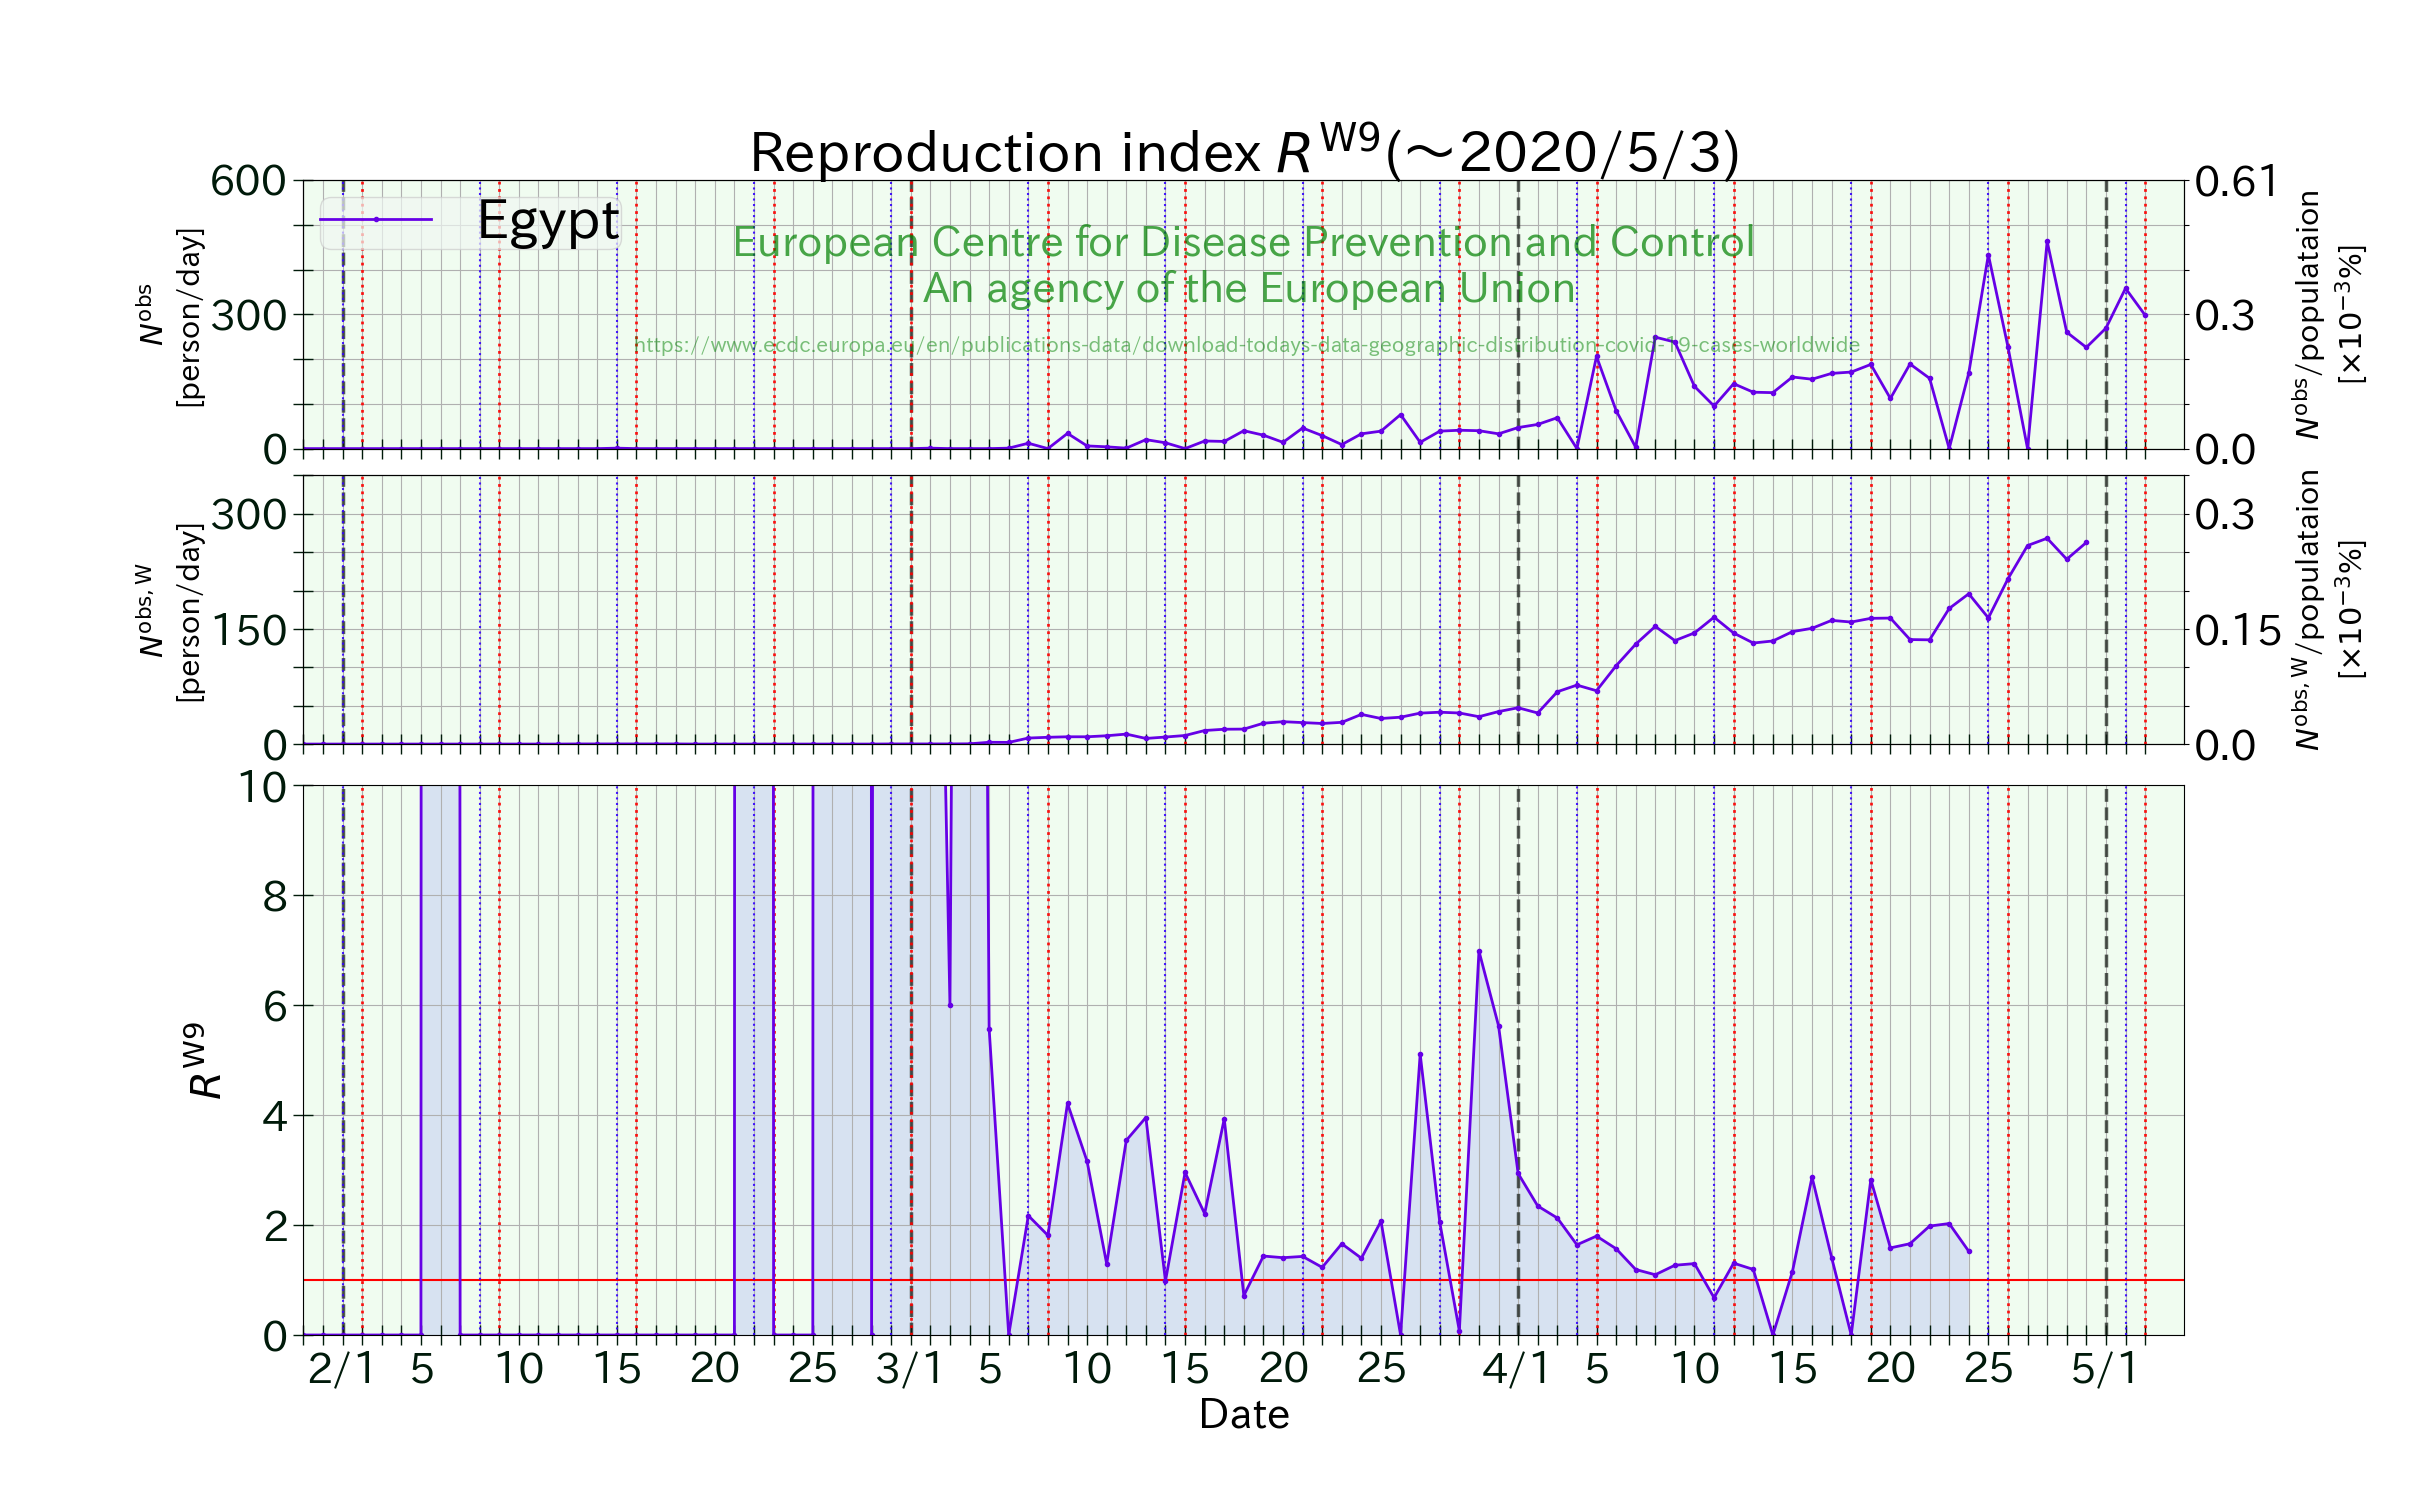
\includegraphics[width=8.9cm]{Egypt.png}
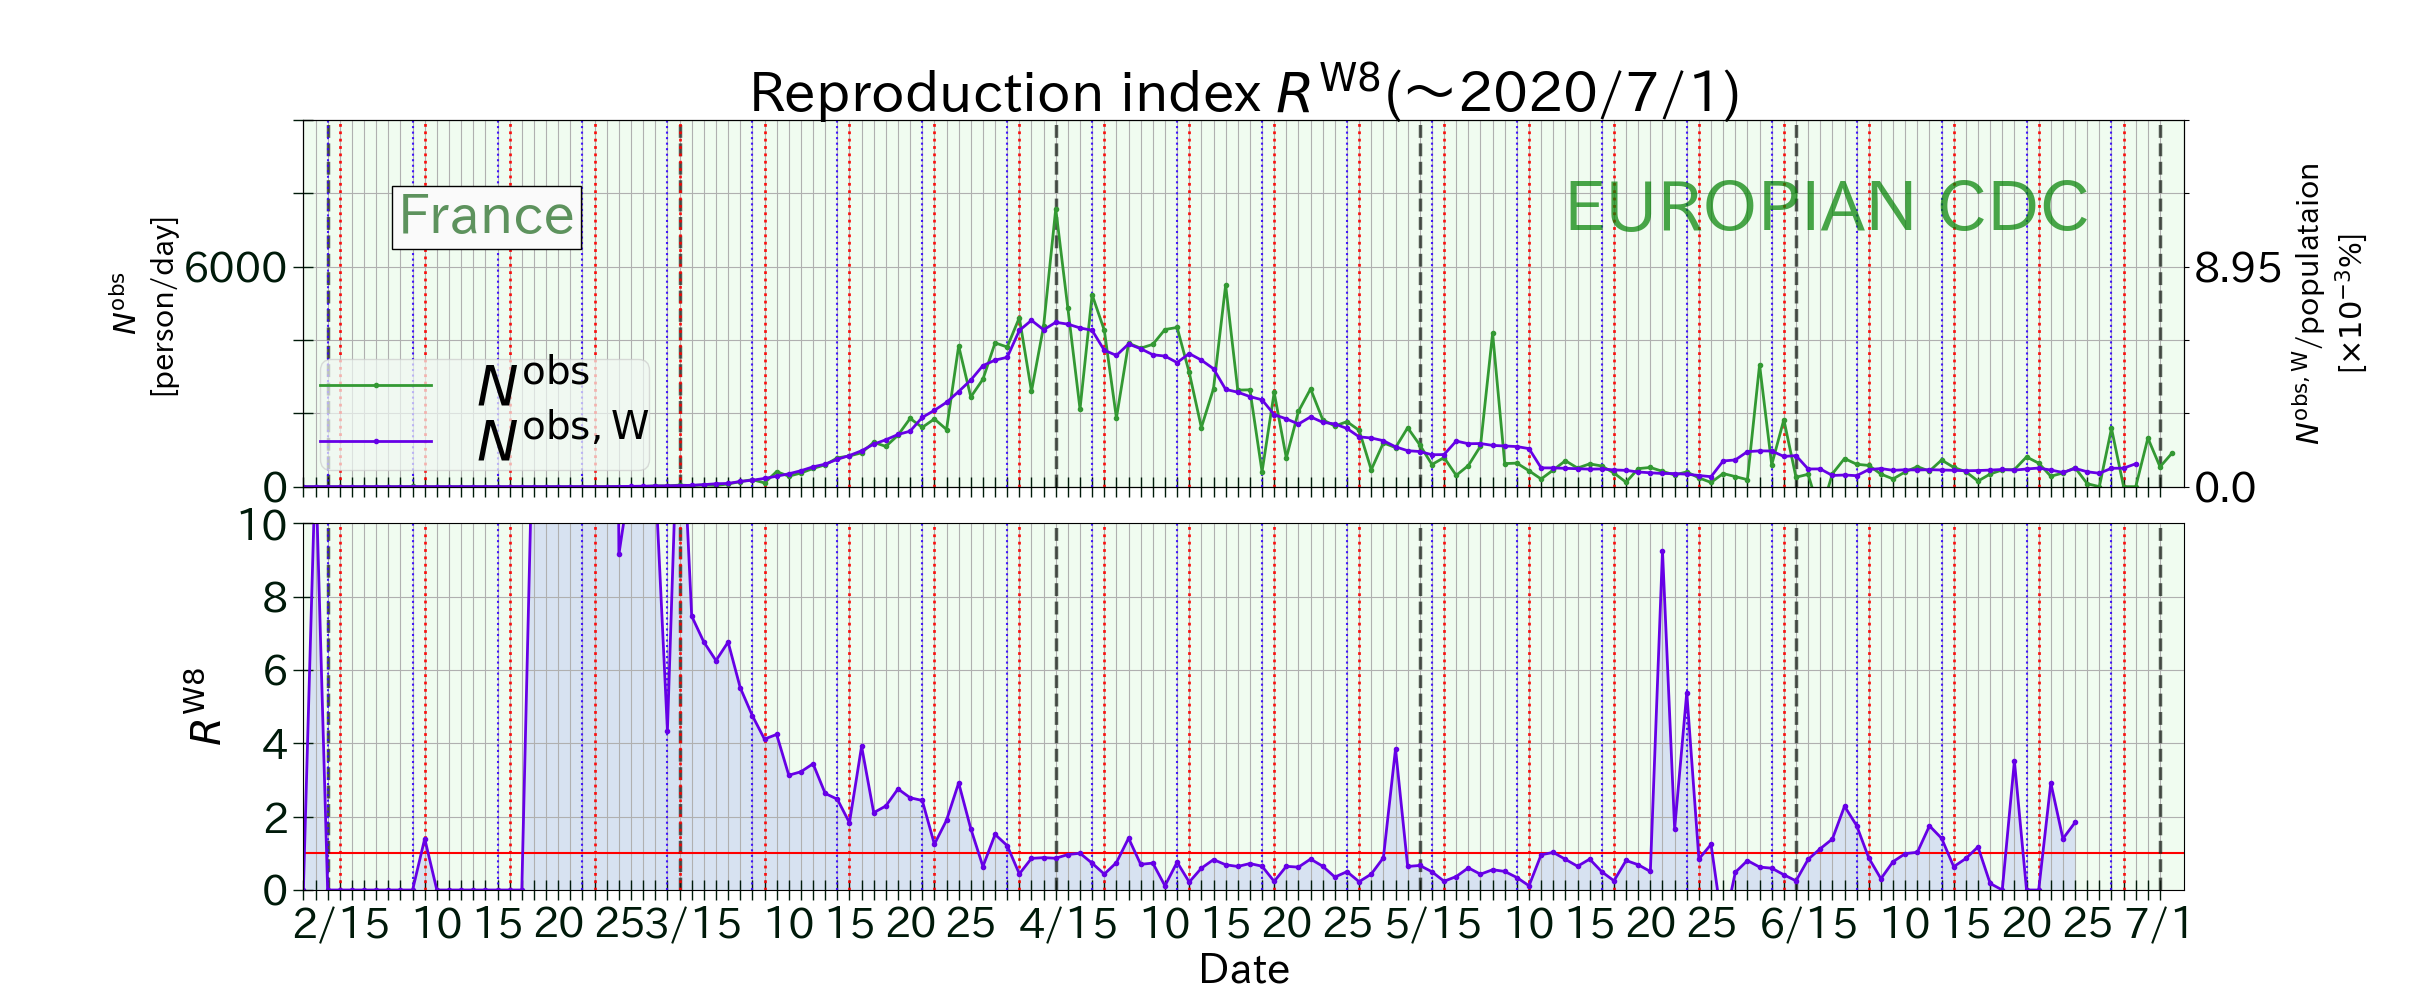
\includegraphics[width=8.9cm]{France.png}
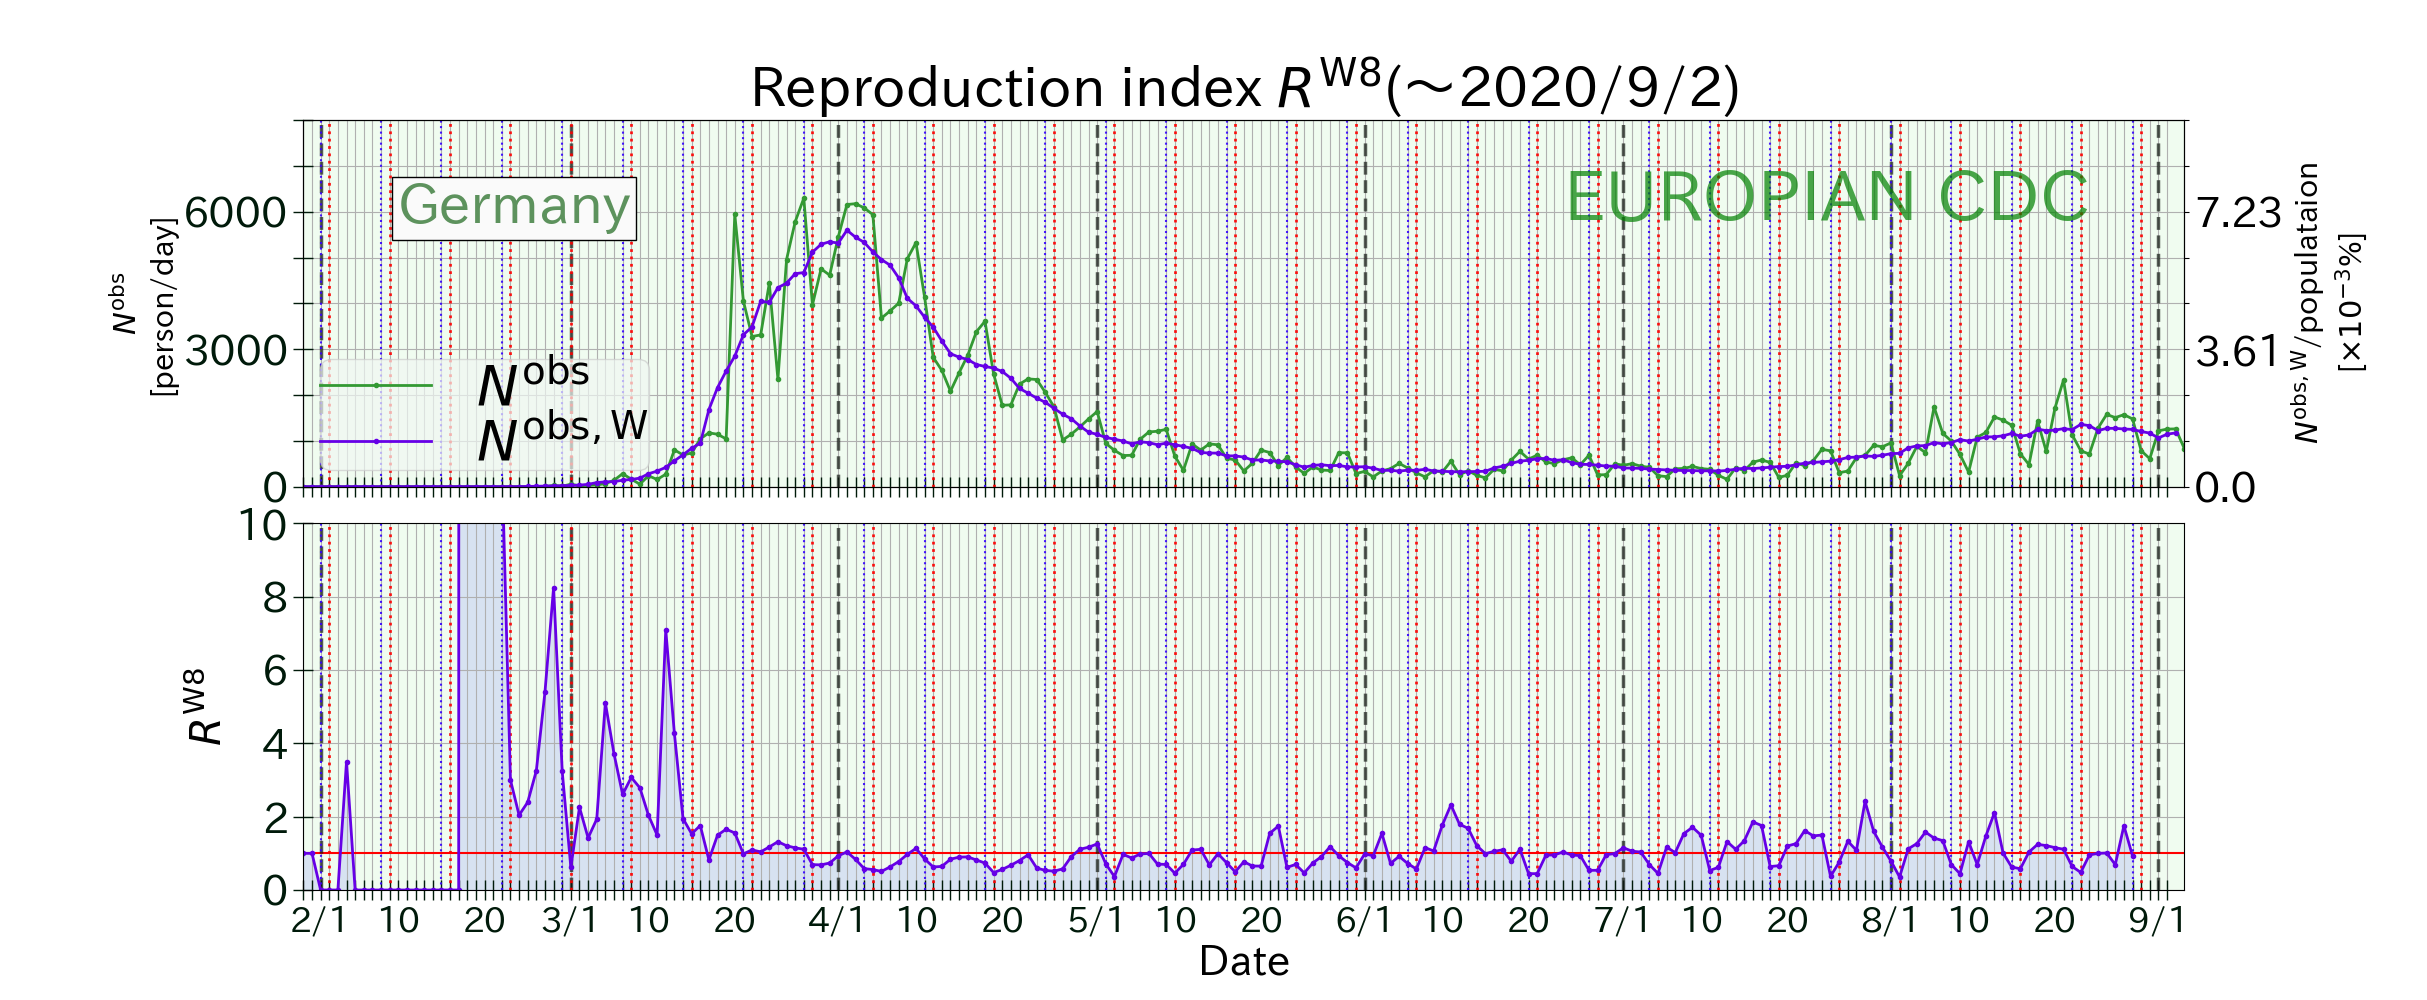
\includegraphics[width=8.9cm]{Germany.png}
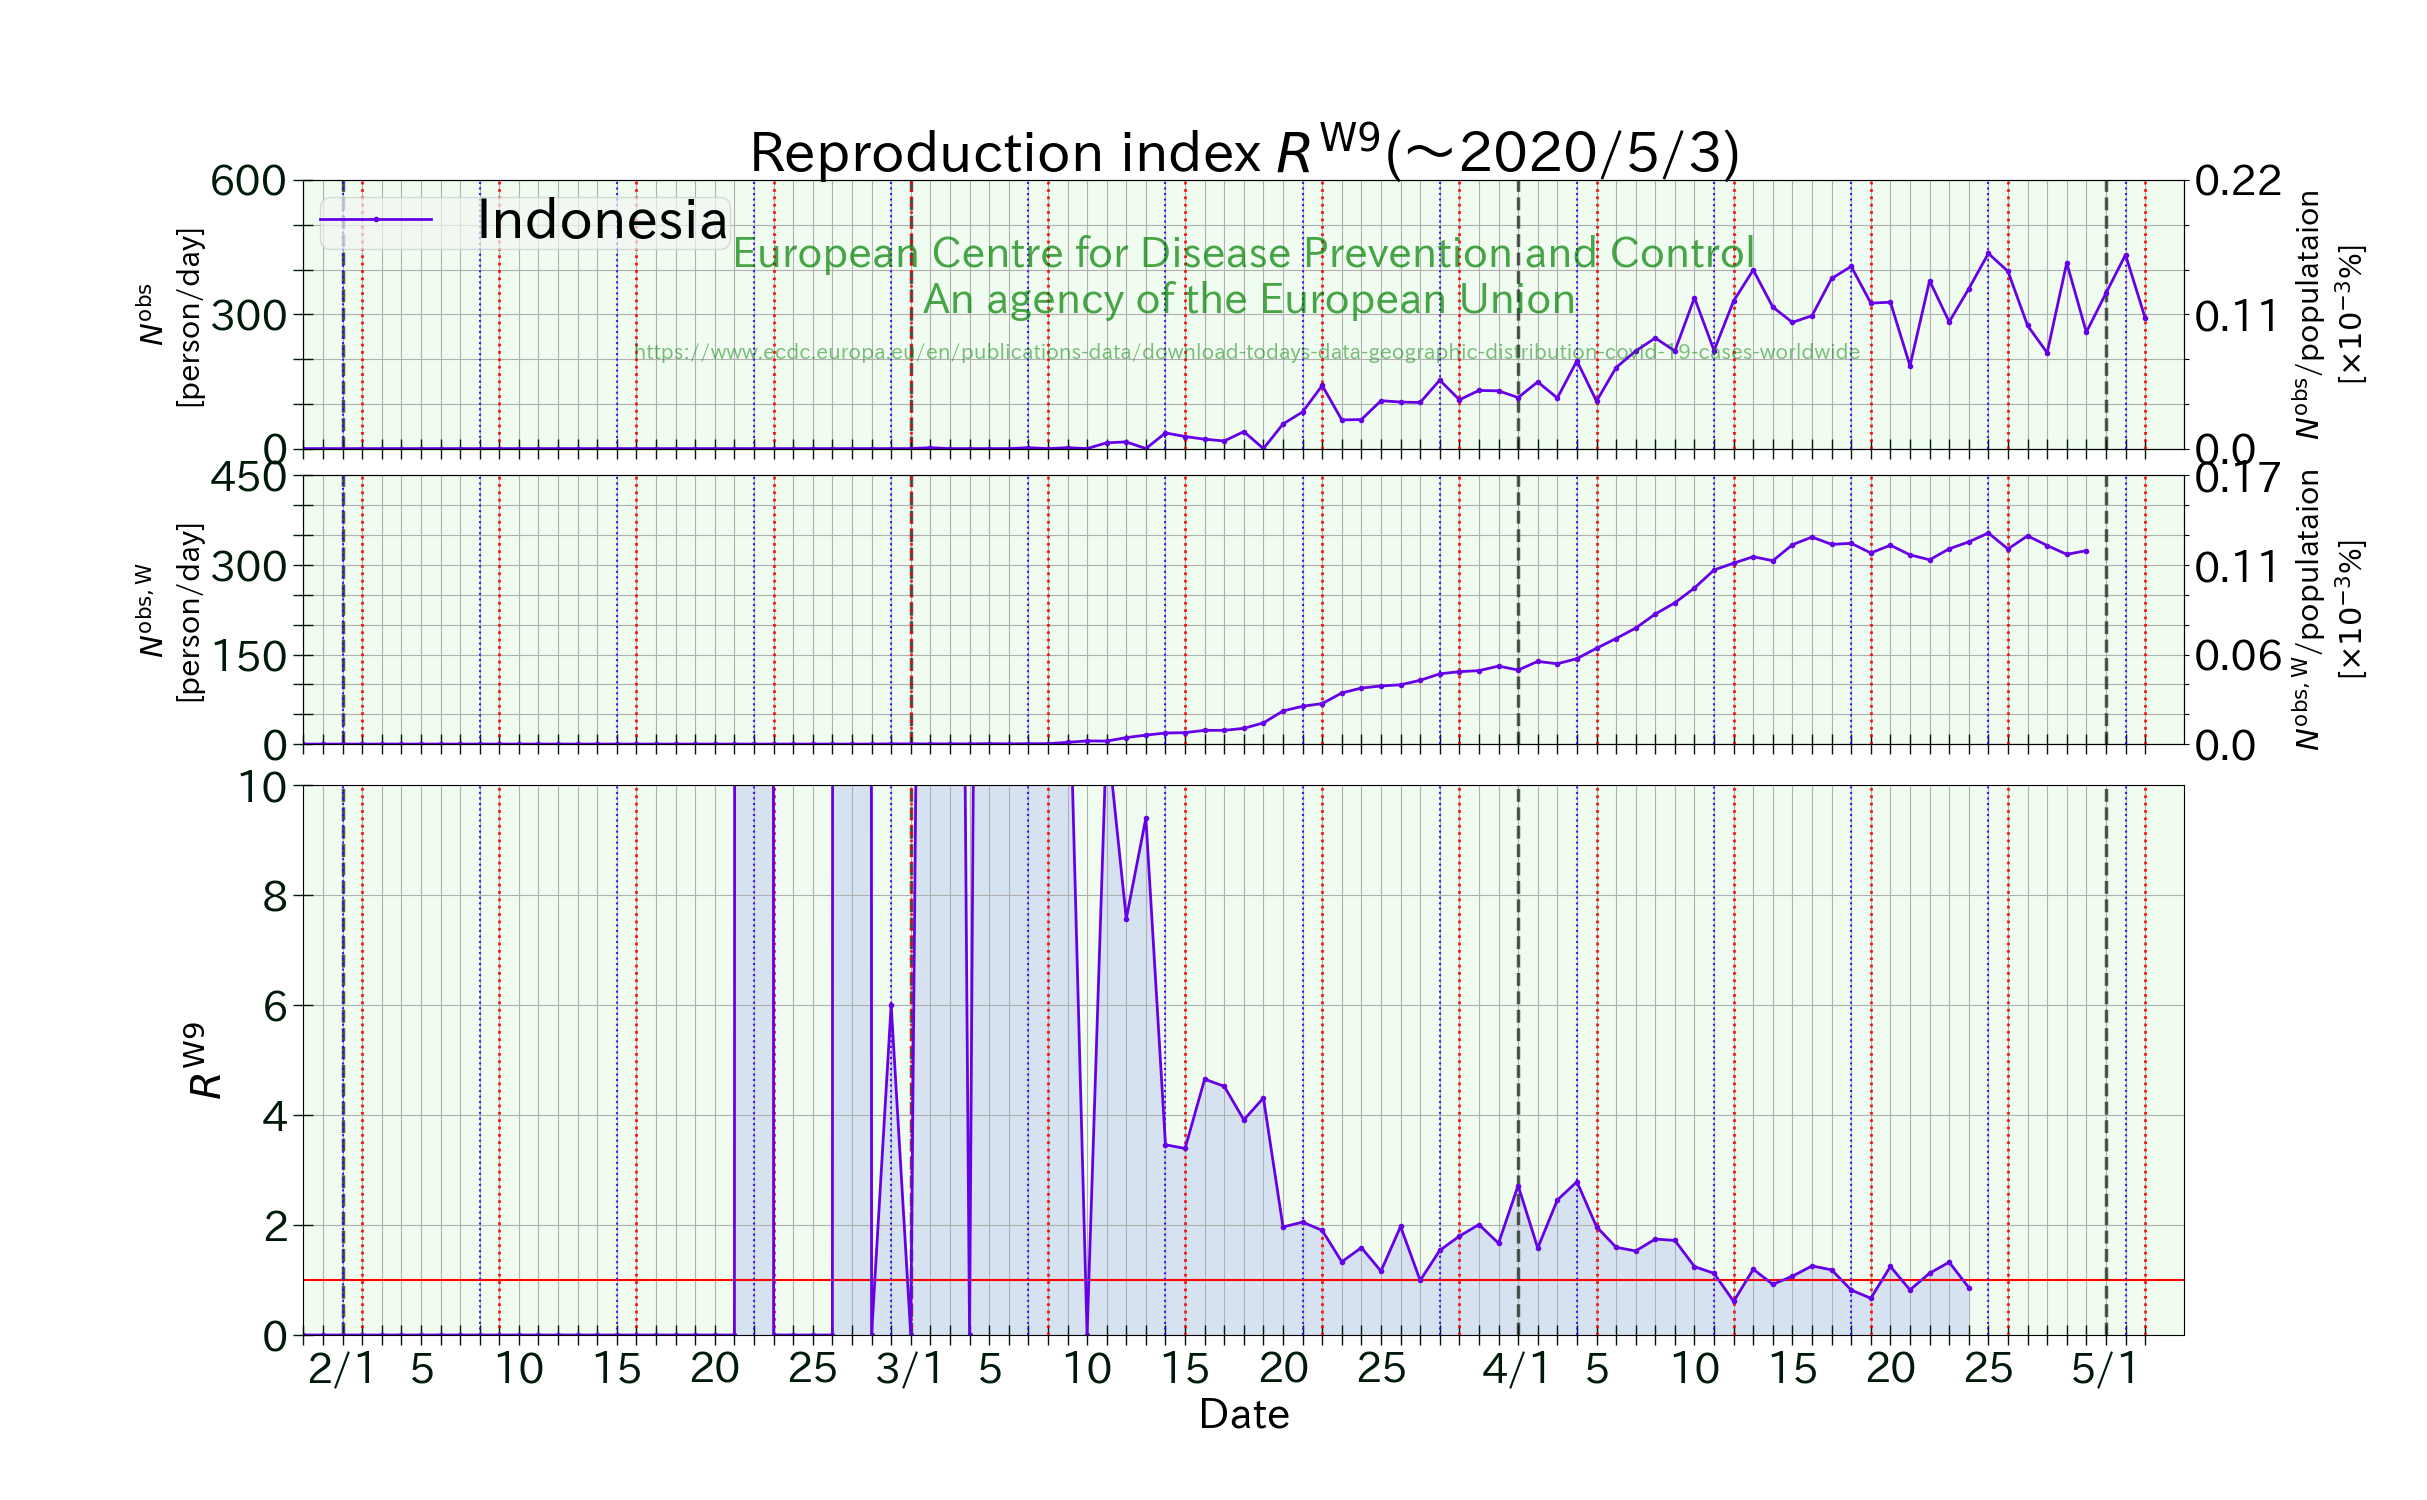
\includegraphics[width=8.9cm]{Indonesia.png}
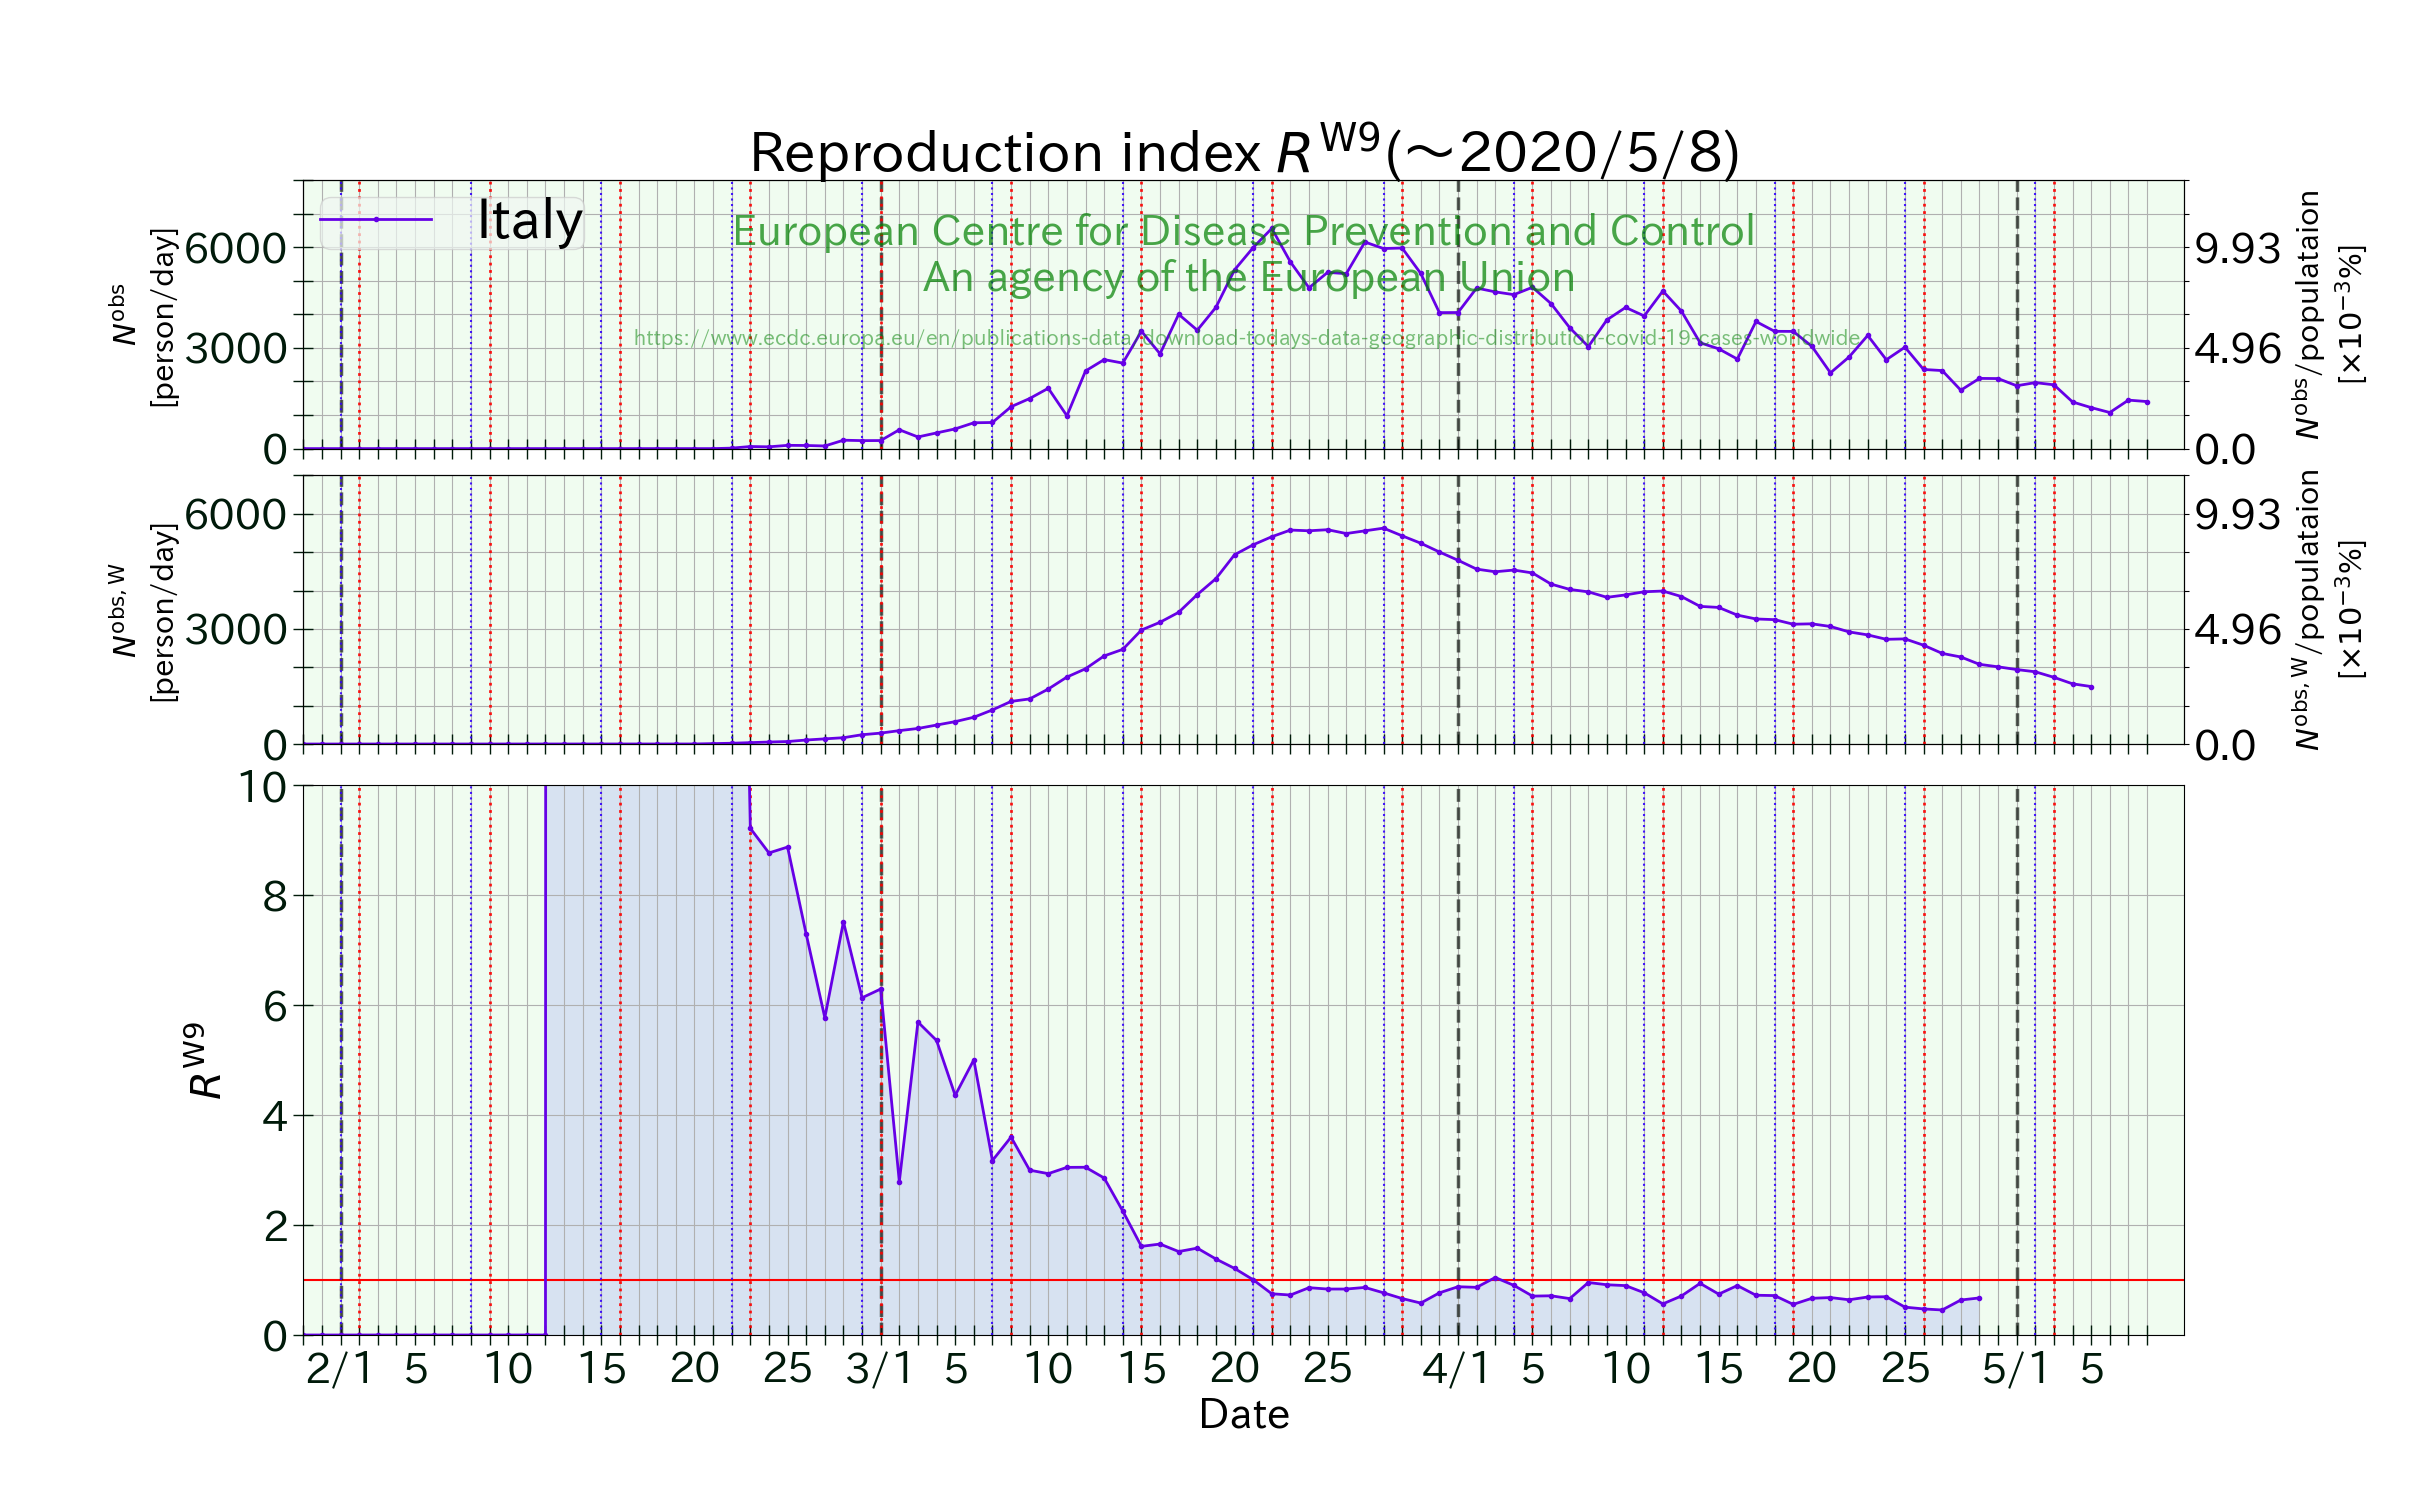
\includegraphics[width=8.9cm]{Italy.png}
 \caption{In the top panel, we show the number of new cases $N^{\rm obs}(i)$.
 In the middle panel, we show the weekly average $N^{\rm obs,W}(i)$.
 In the bottom panel, we show the reproduction index $R^{\rm W9}(i)$,
 where hatch areas below data lines as a guide of eyes.}
 \end{figure*}

\begin{figure*}[ht]
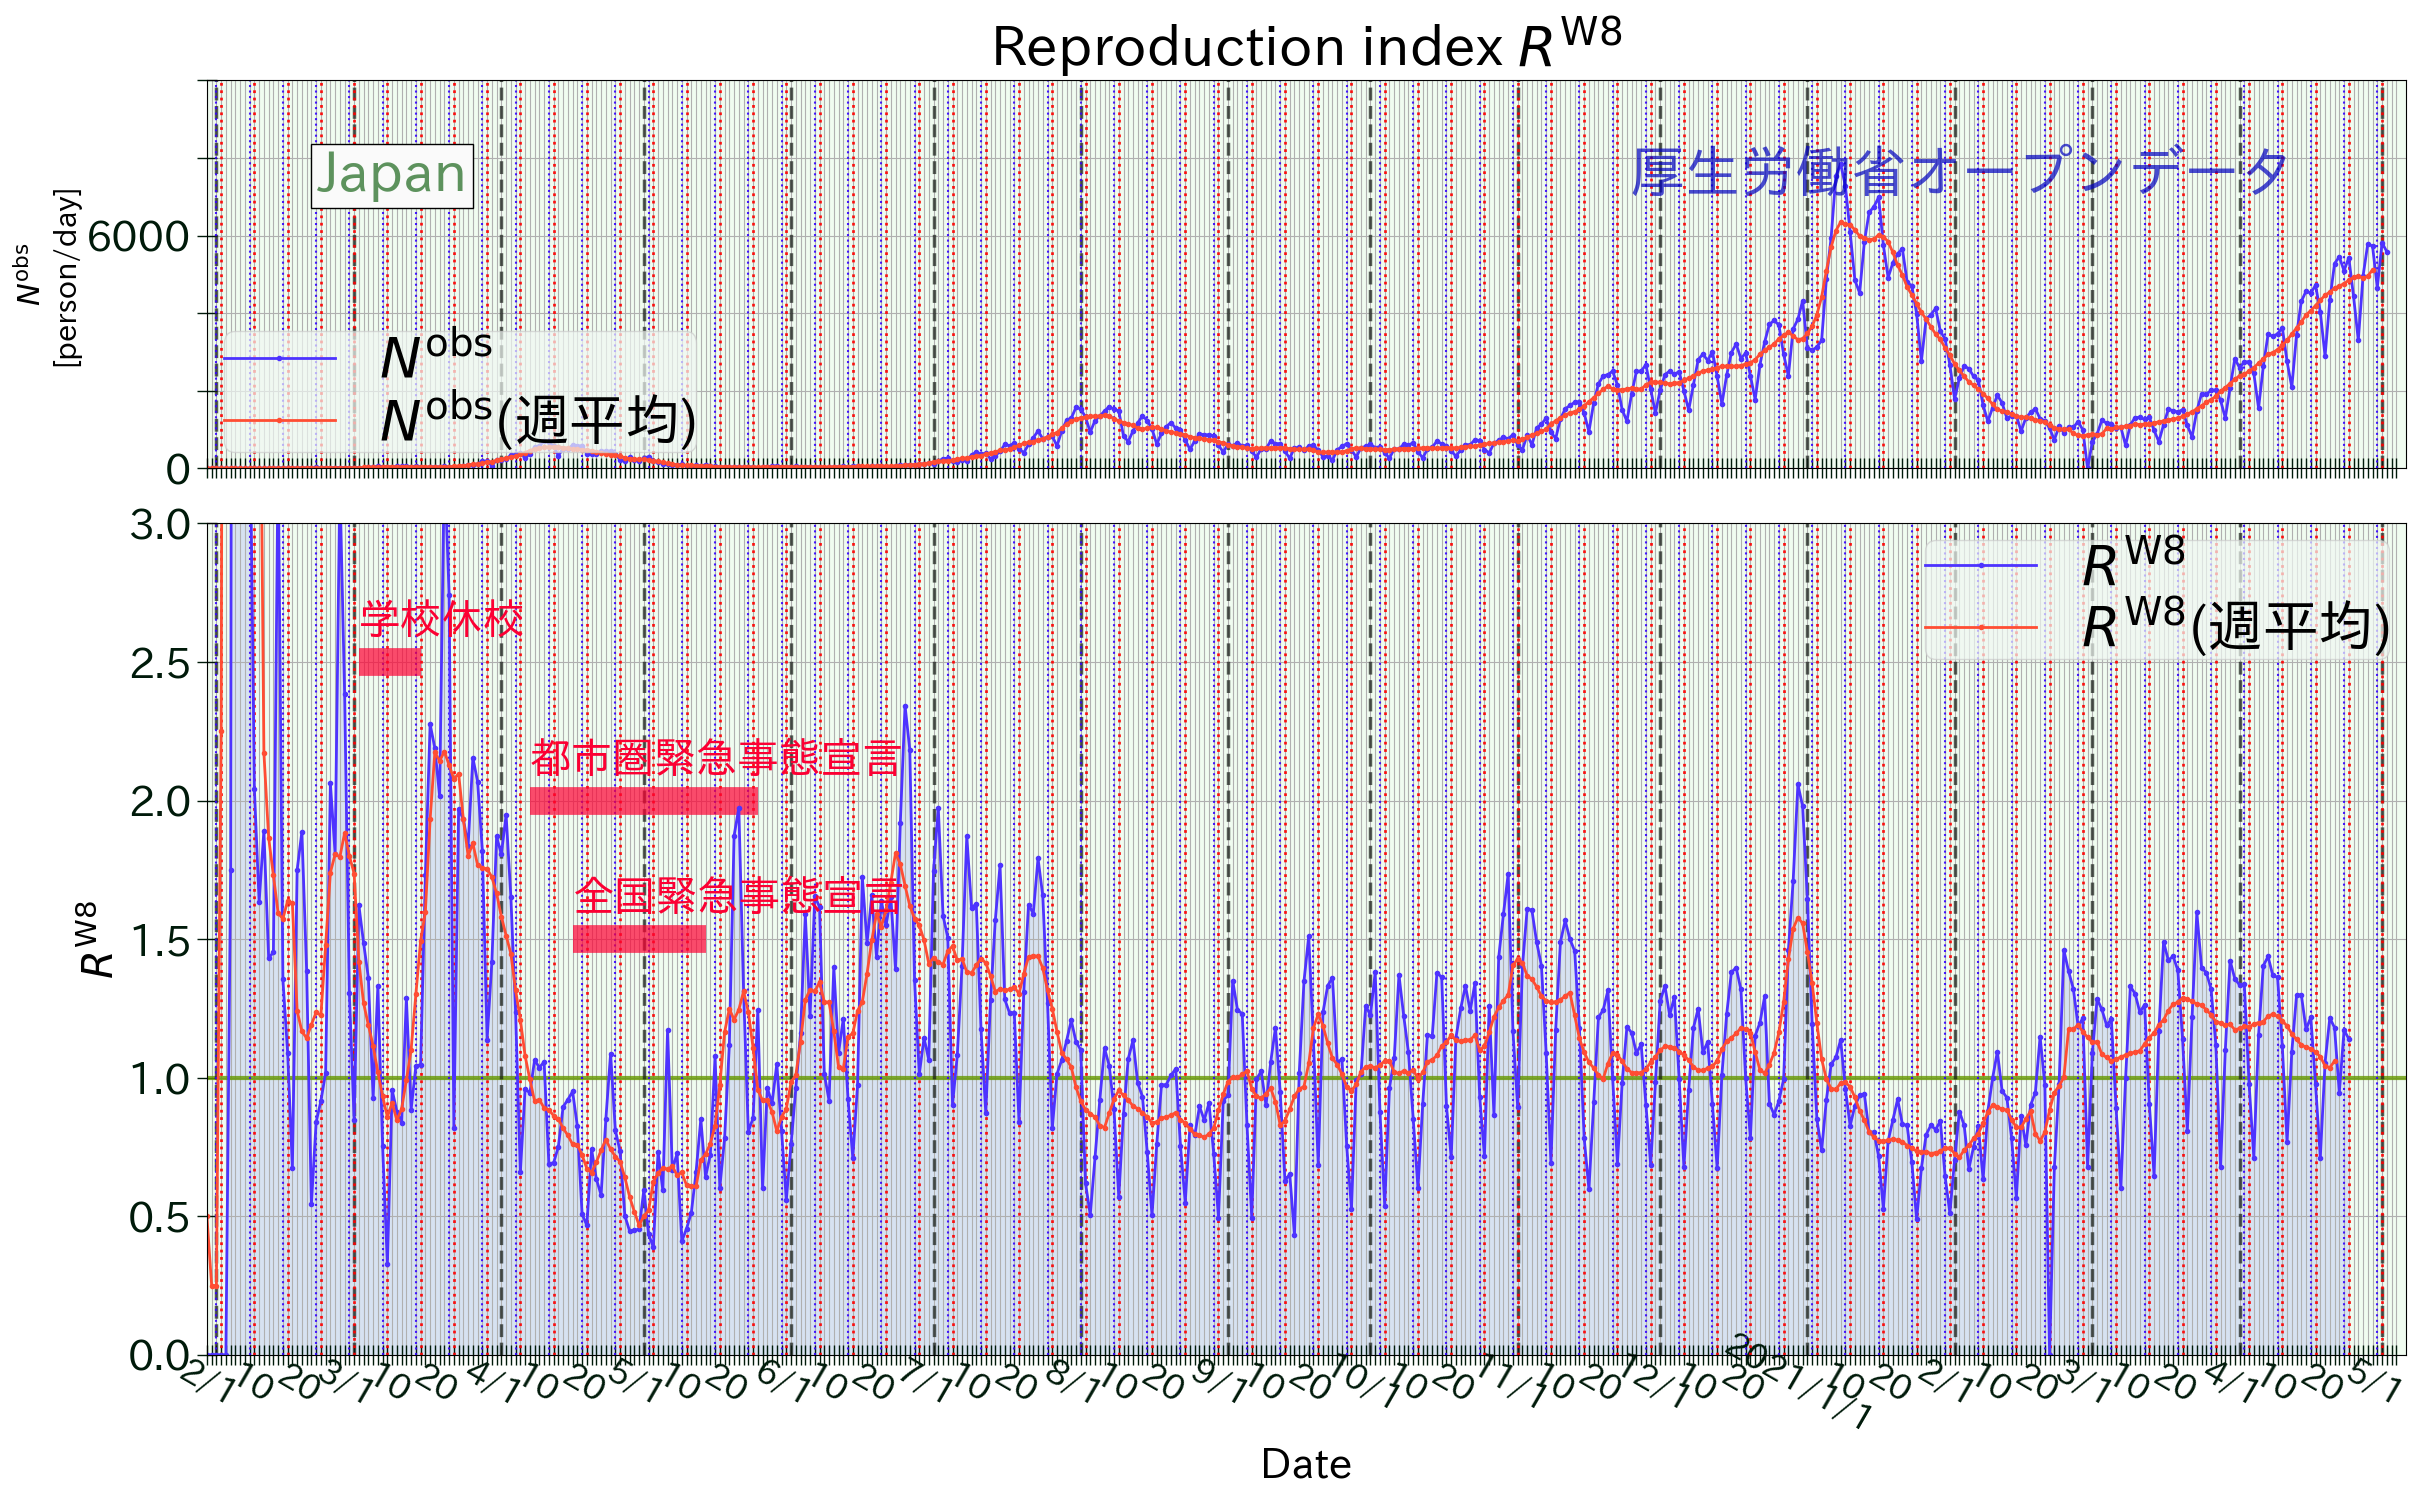
\includegraphics[width=8.9cm]{Japan.png}
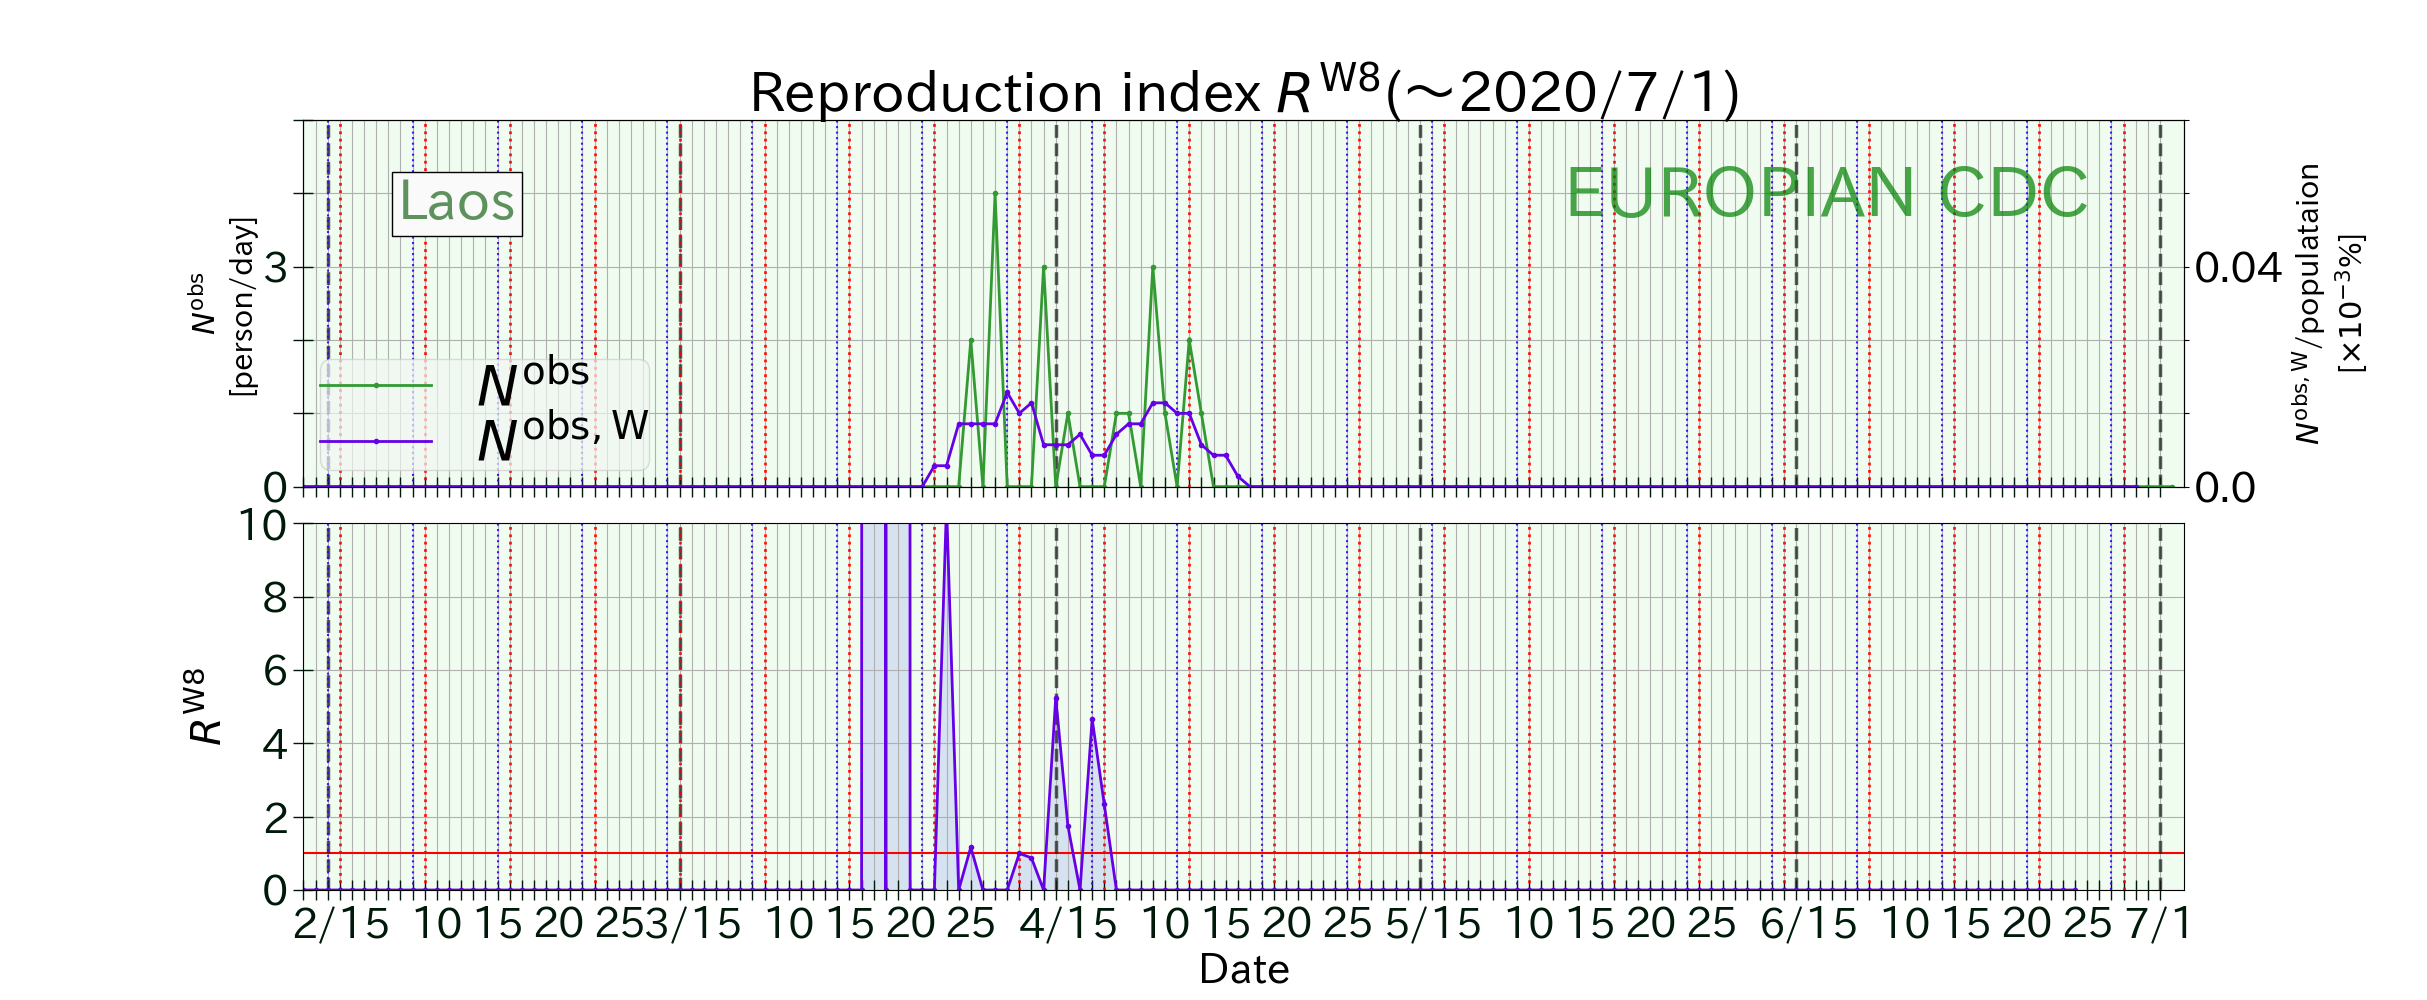
\includegraphics[width=8.9cm]{Laos.png}
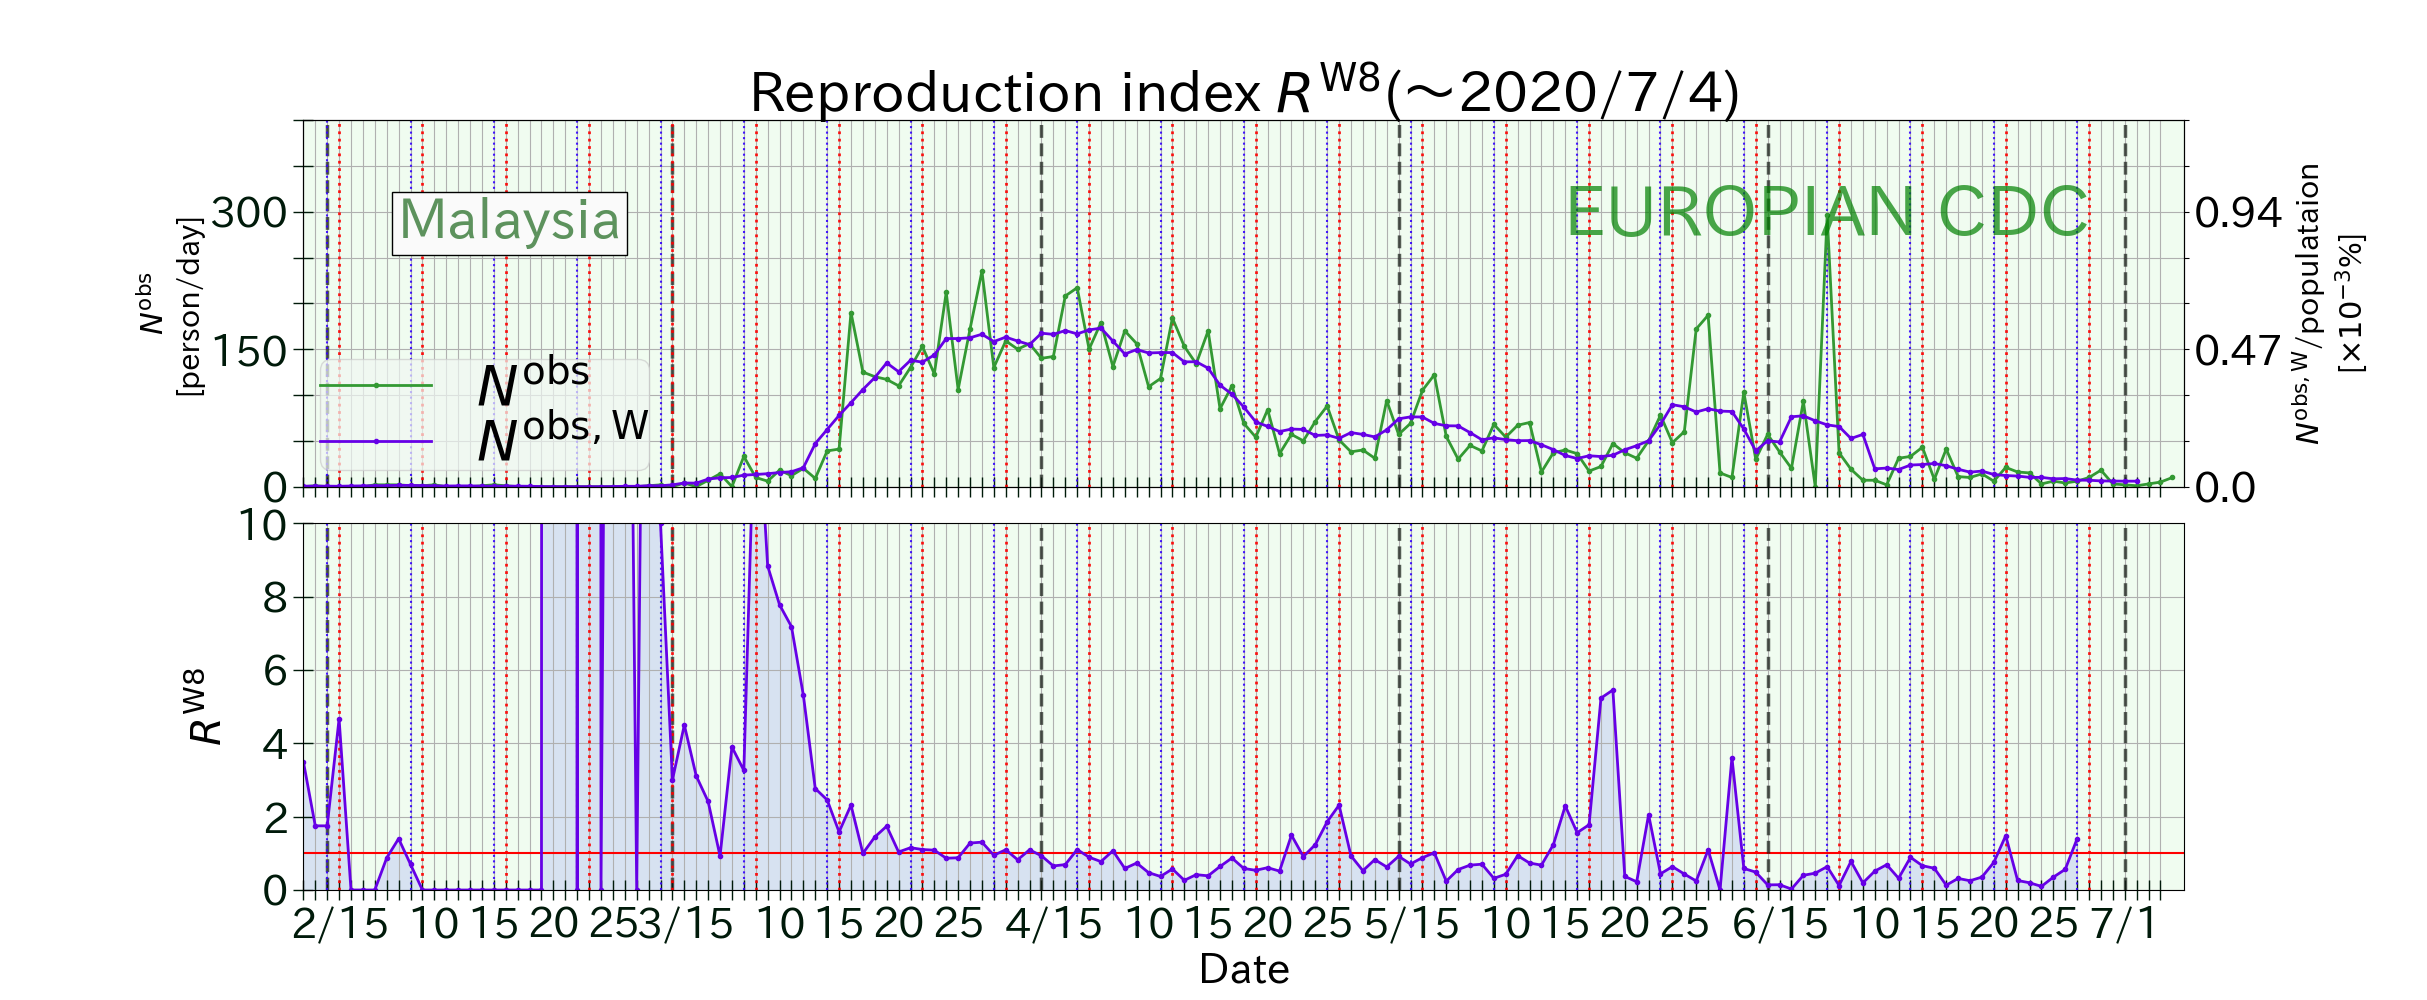
\includegraphics[width=8.9cm]{Malaysia.png}
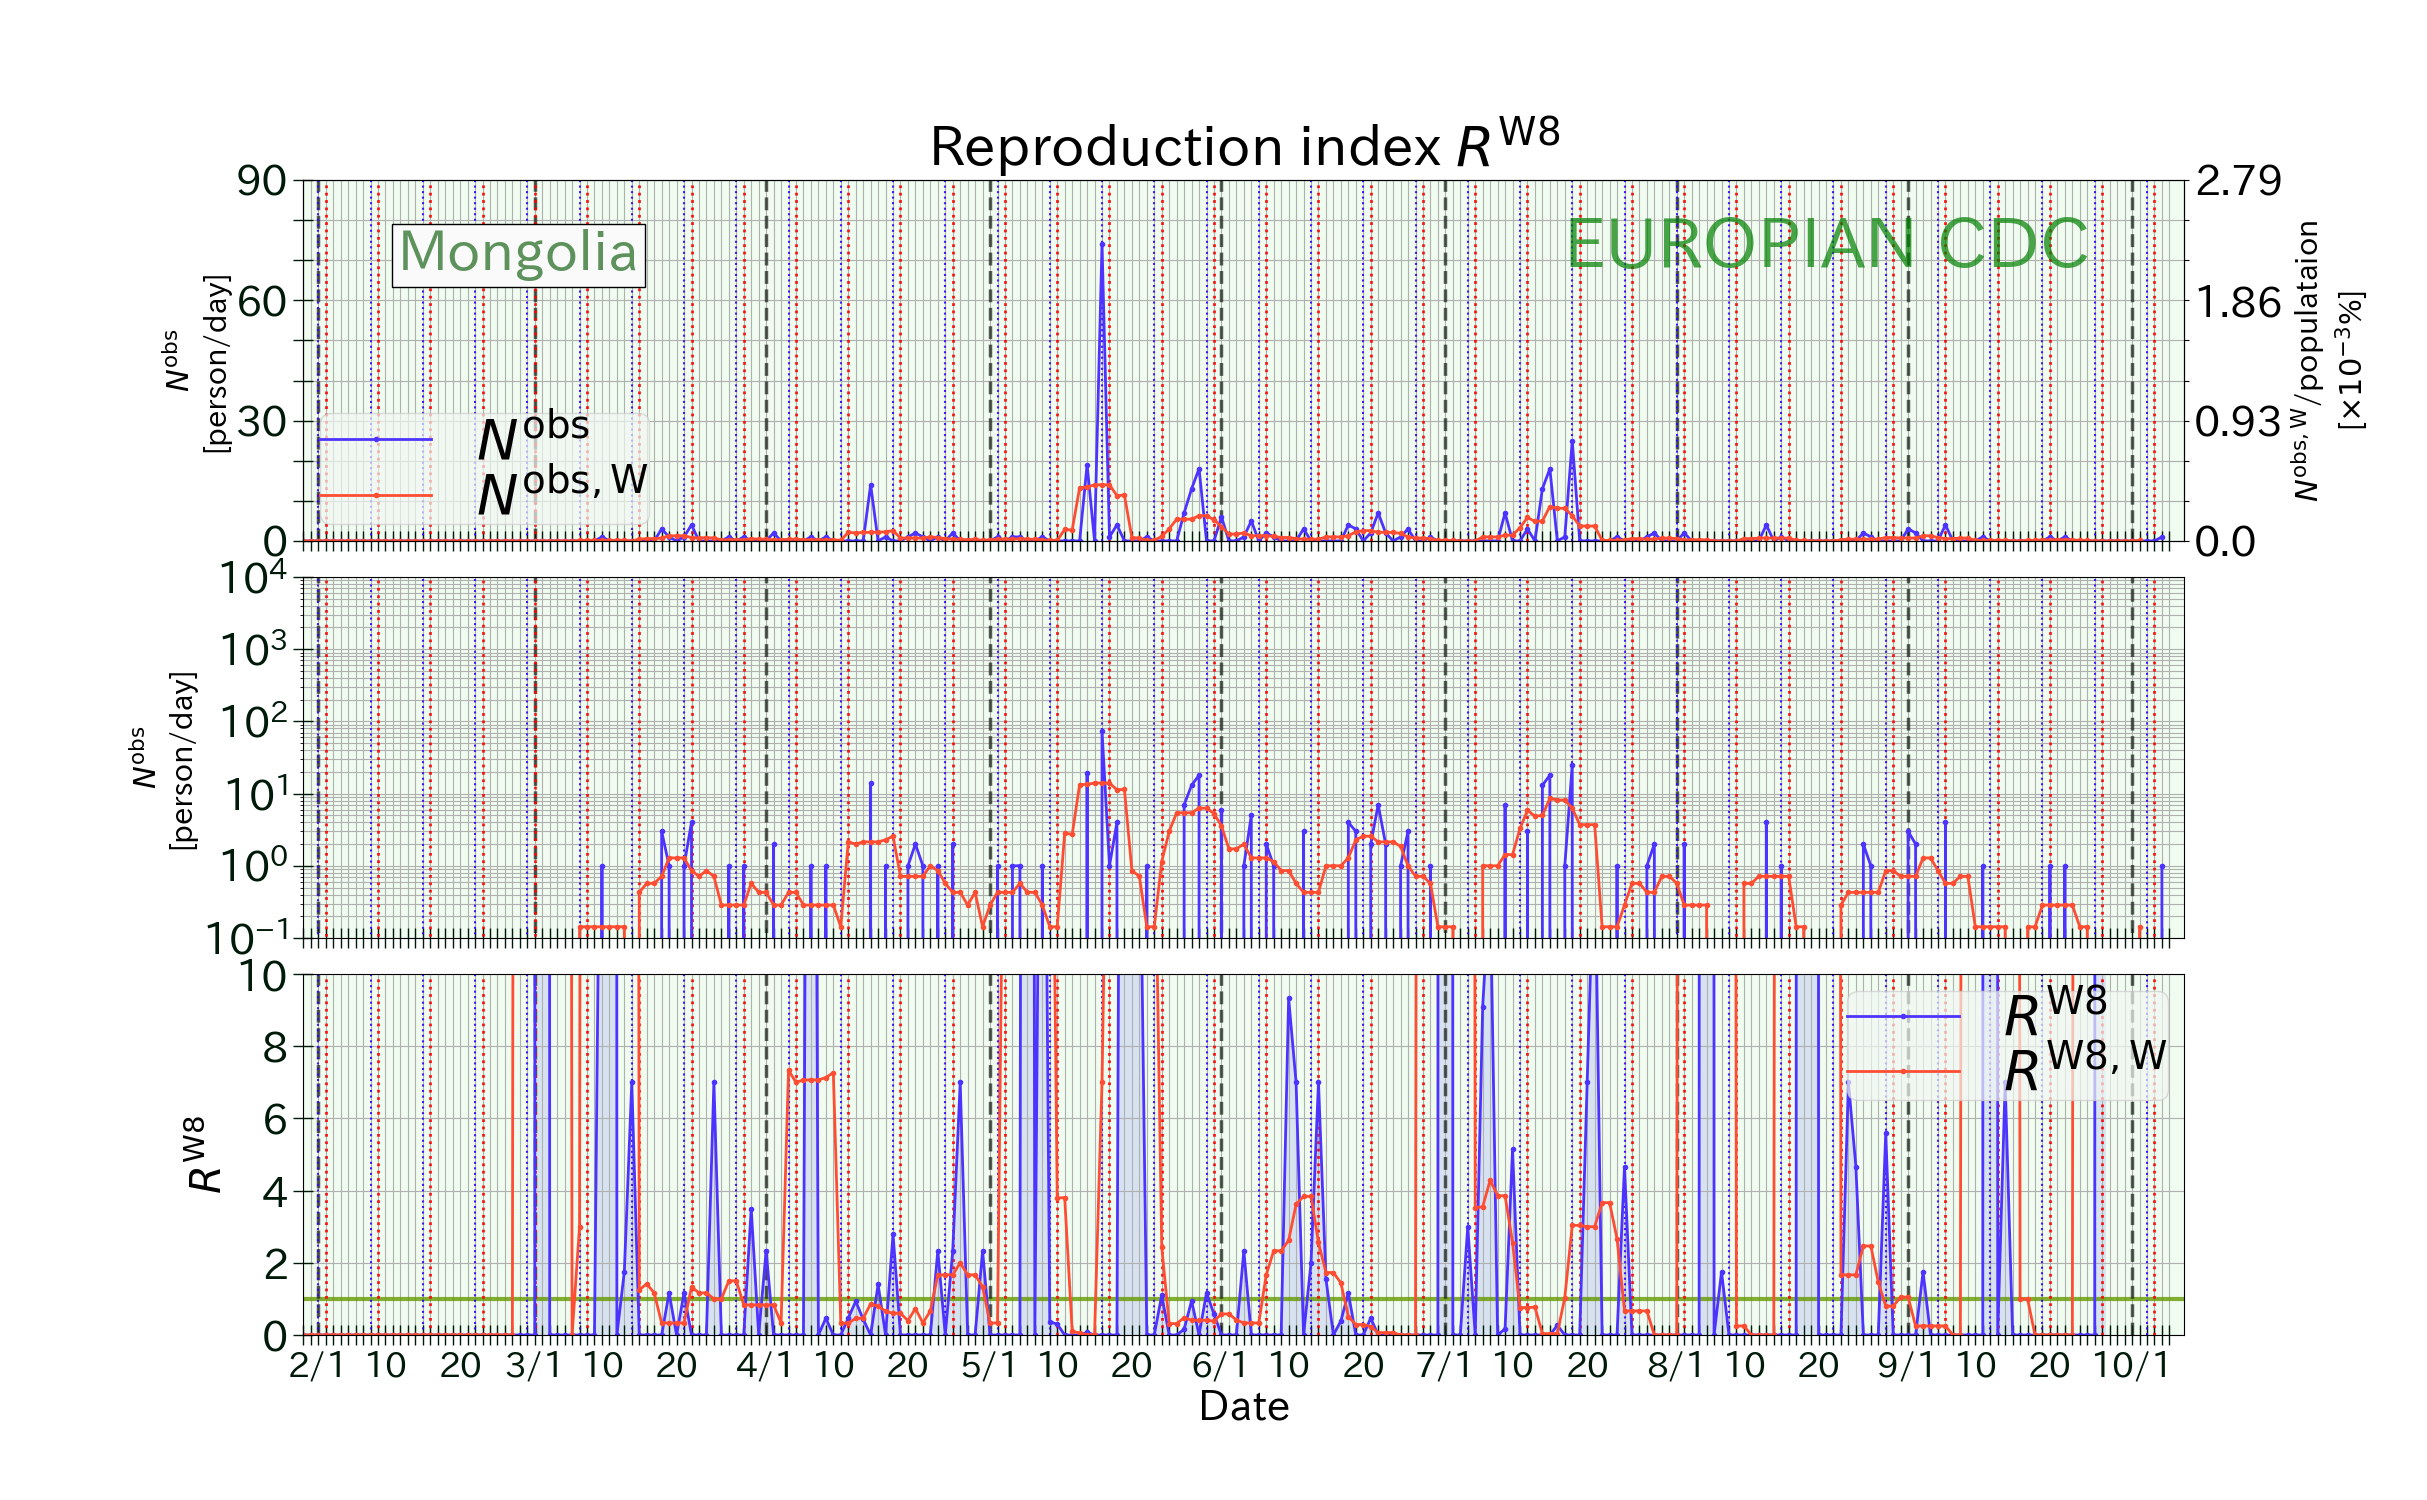
\includegraphics[width=8.9cm]{Mongolia.png}
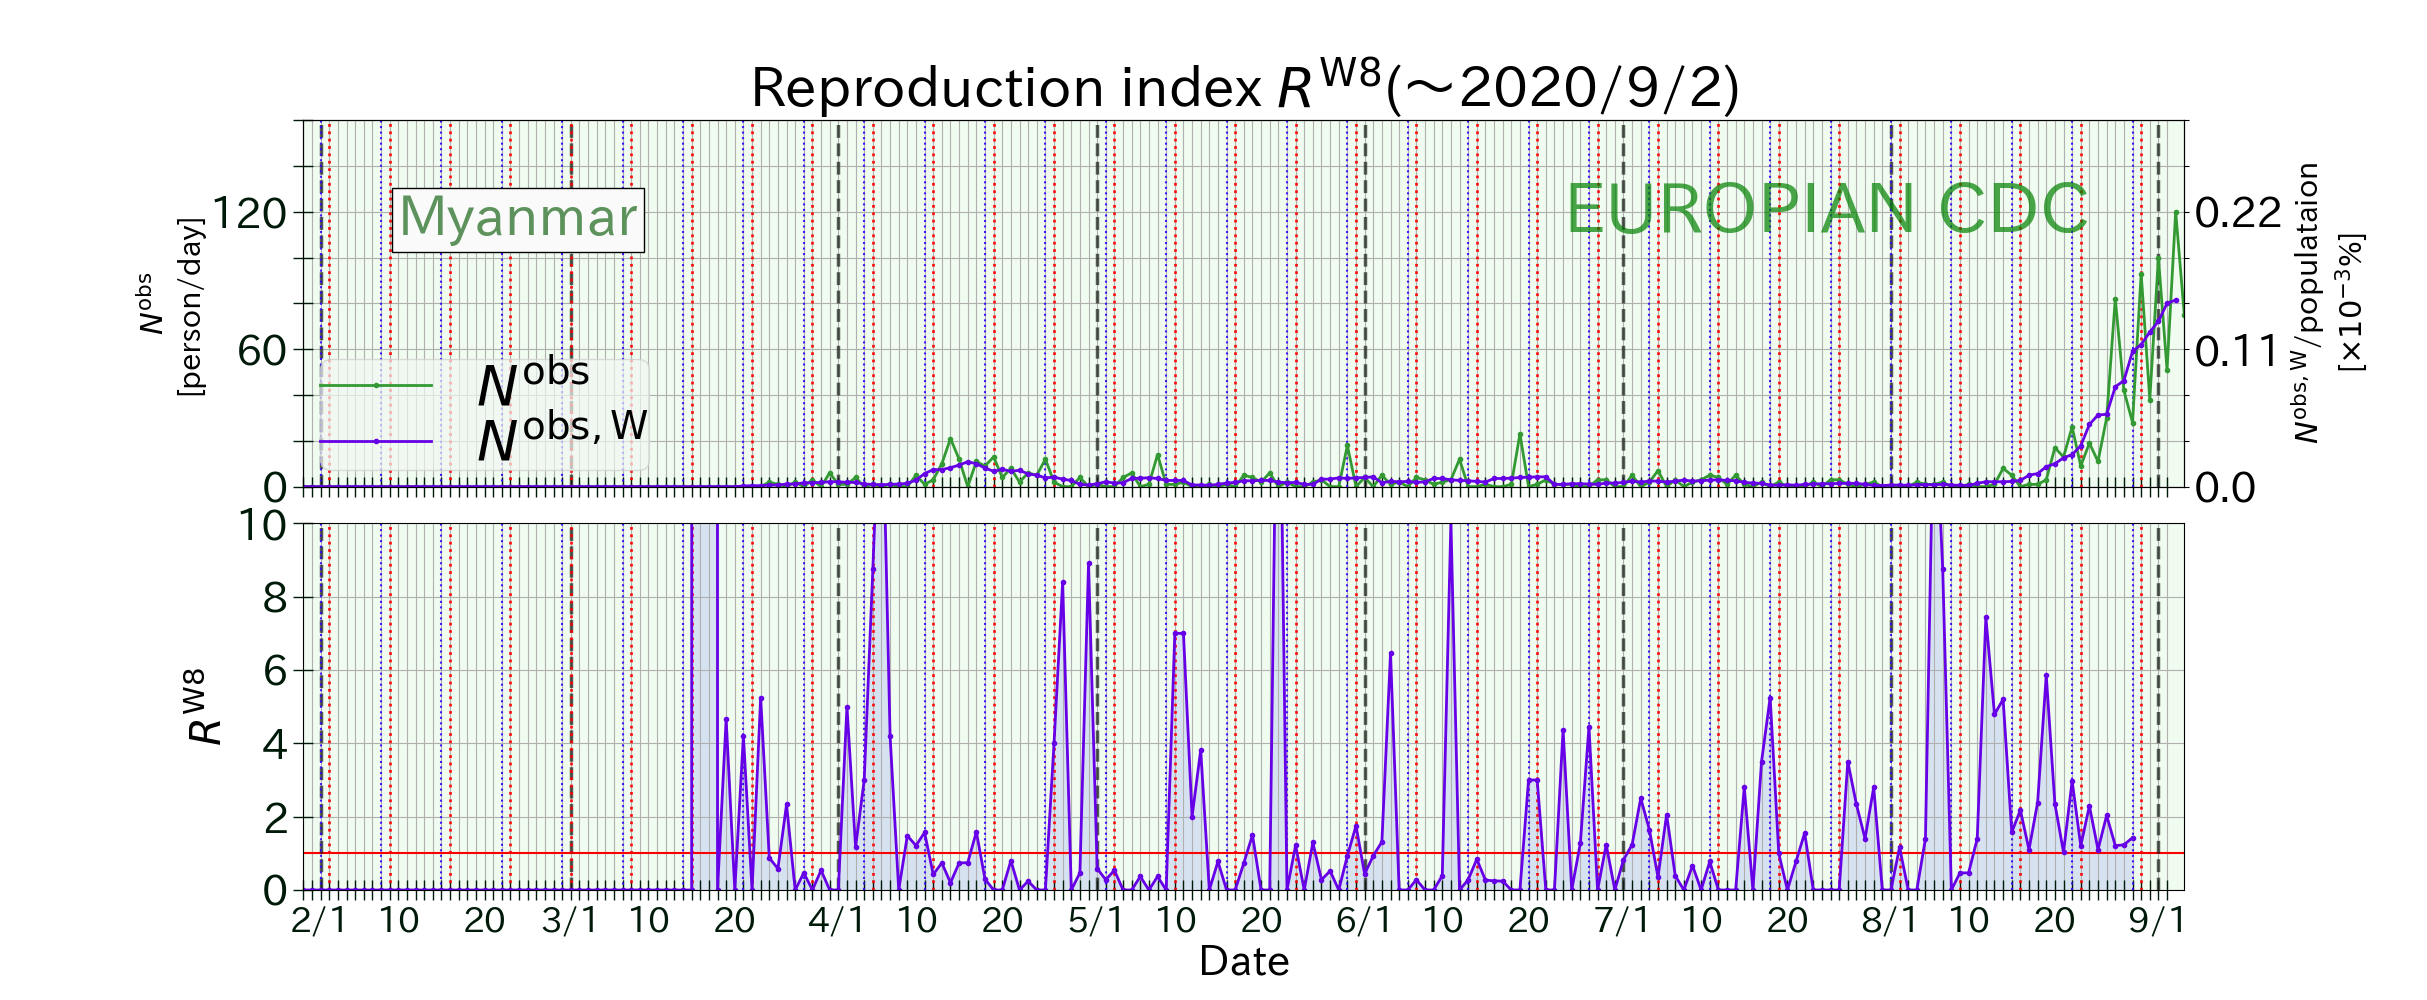
\includegraphics[width=8.9cm]{Myanmar.png}
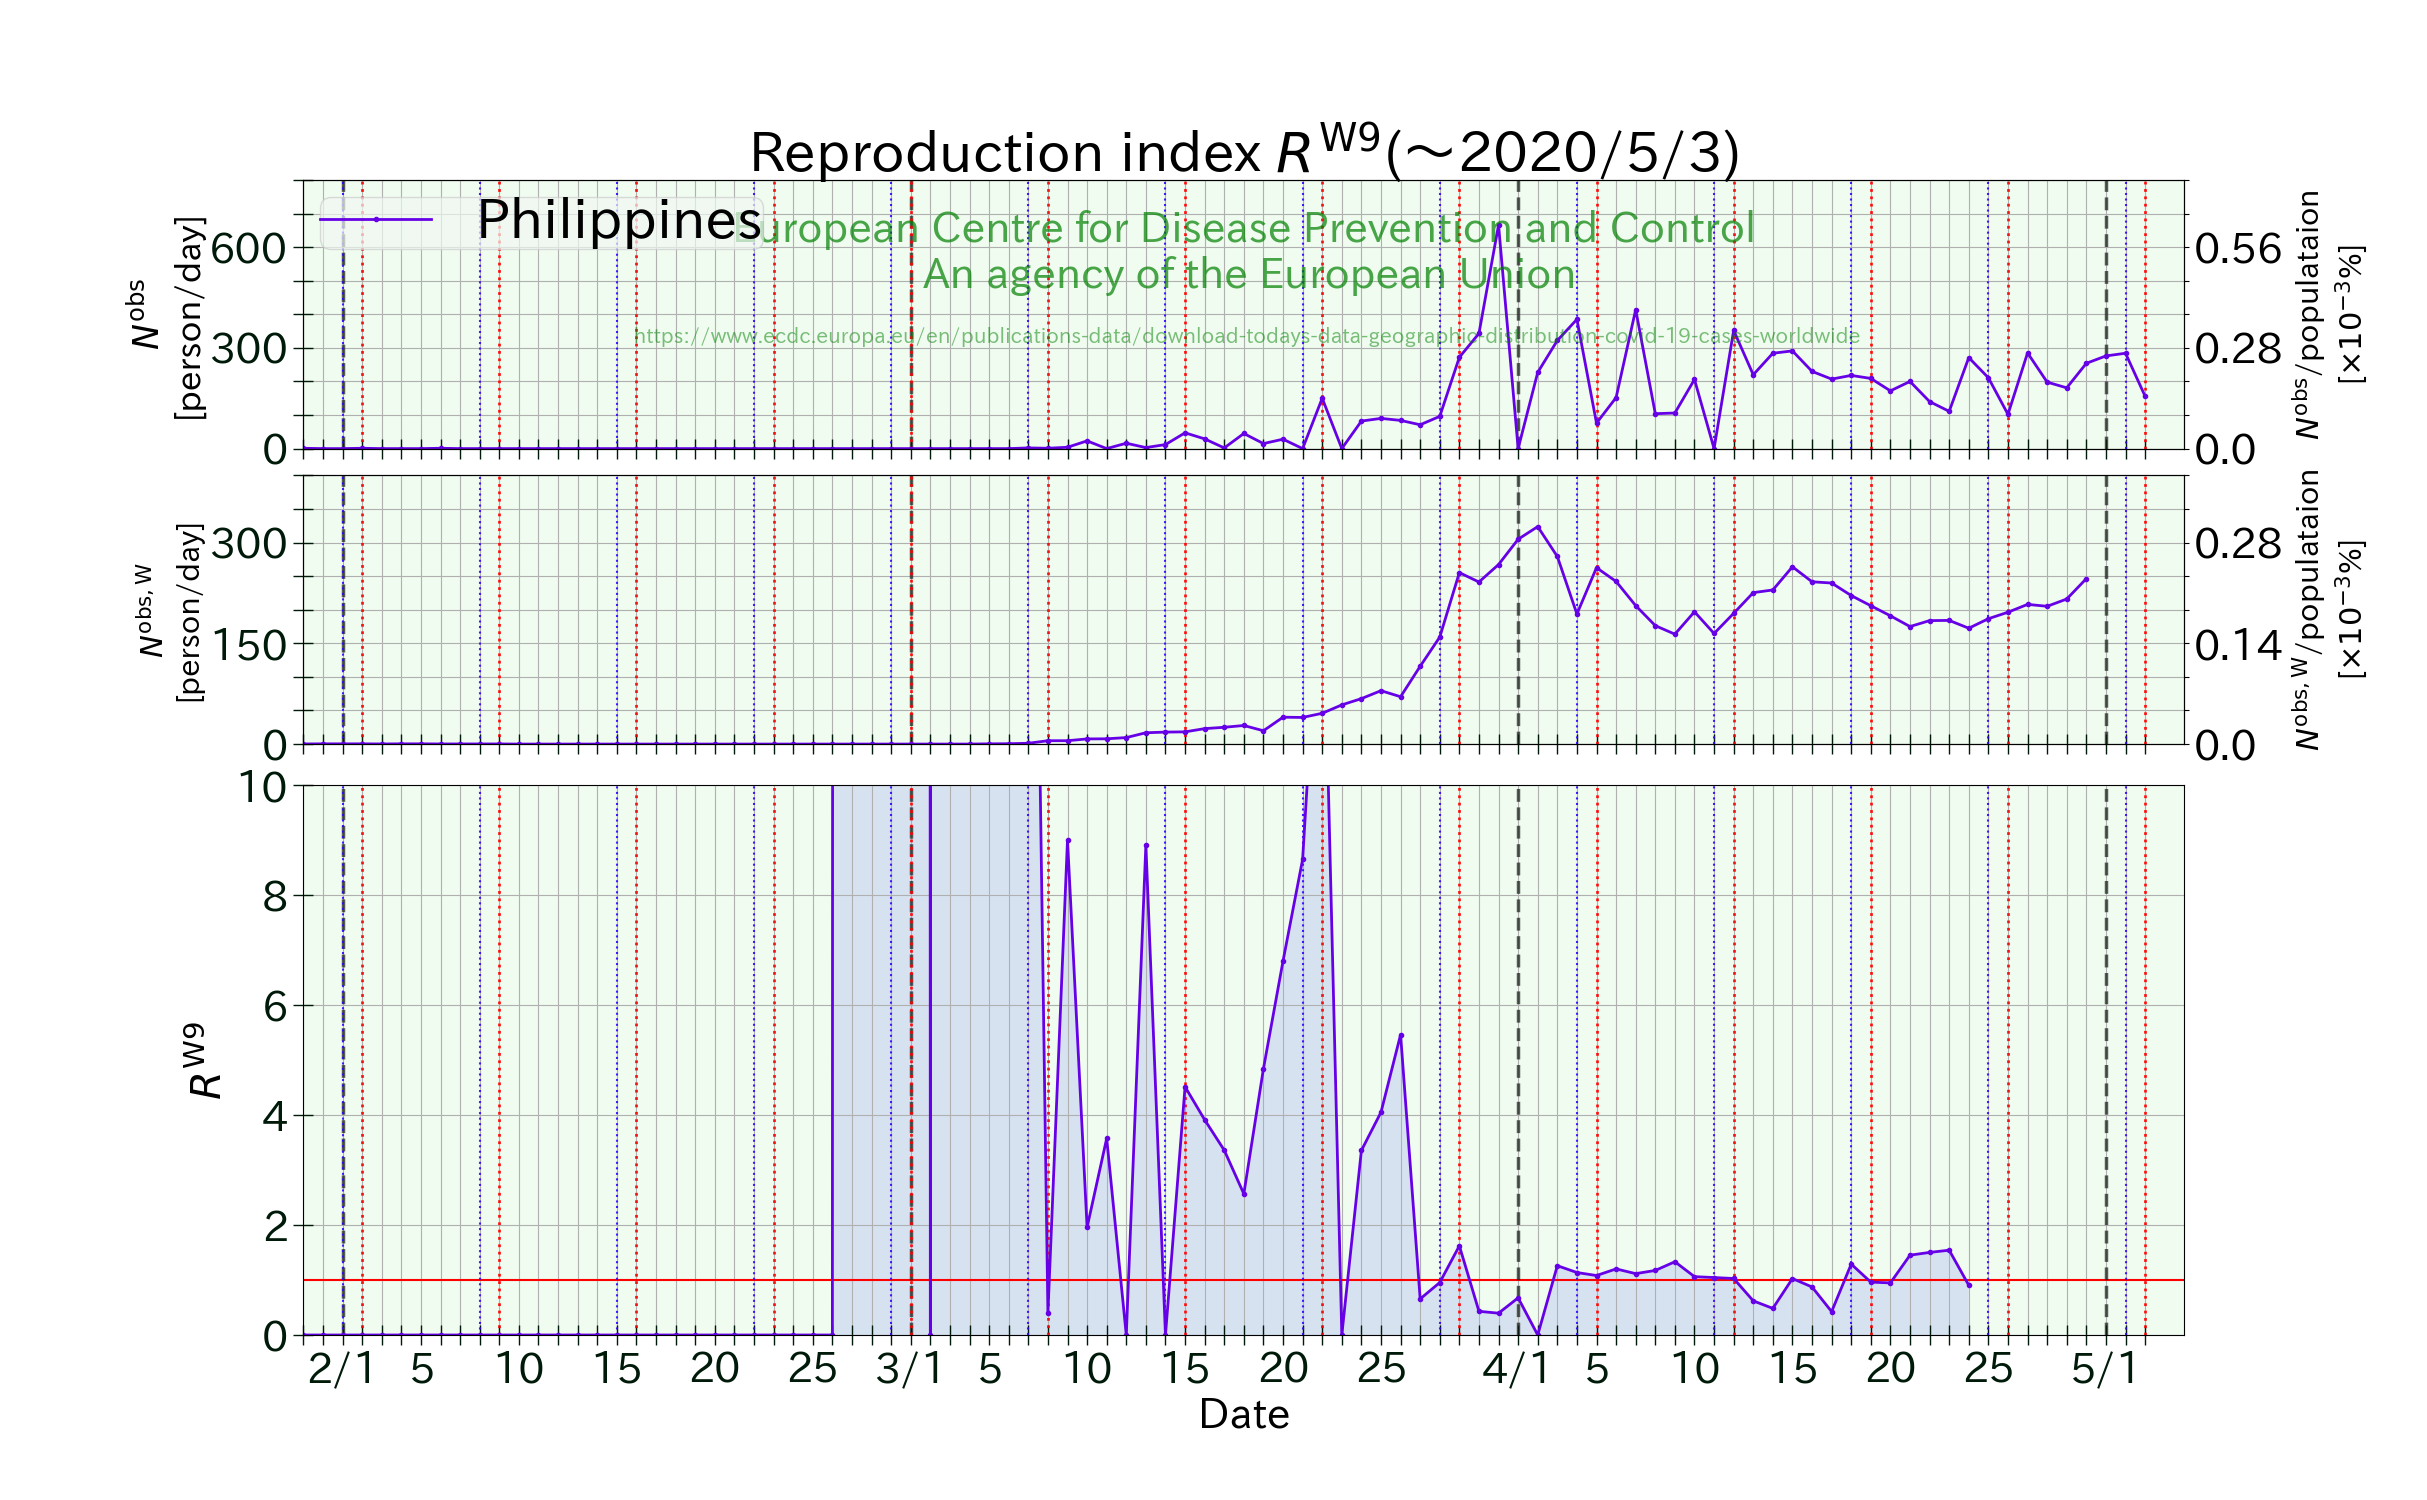
\includegraphics[width=8.9cm]{Philippines.png}
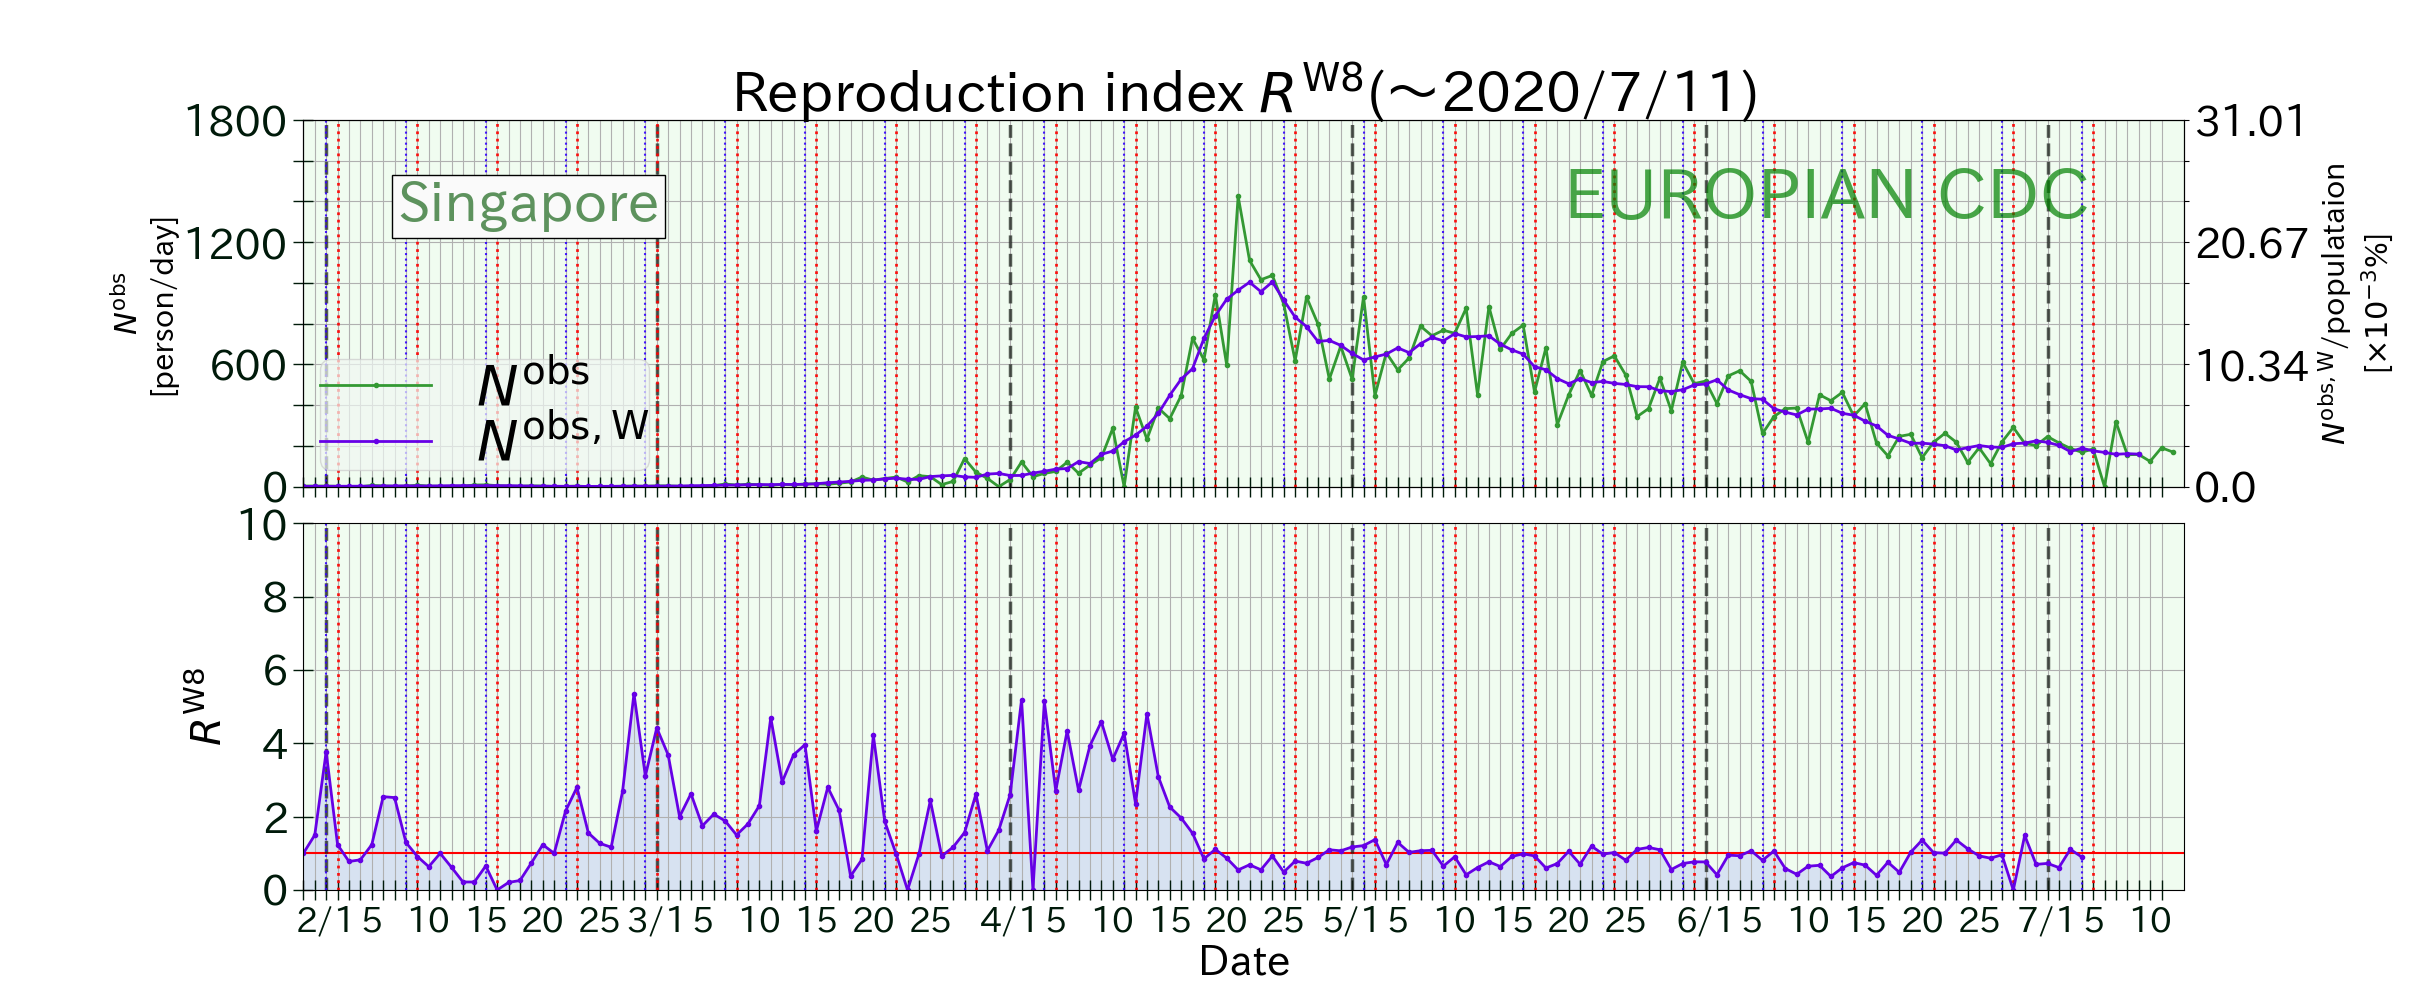
\includegraphics[width=8.9cm]{Singapore.png}
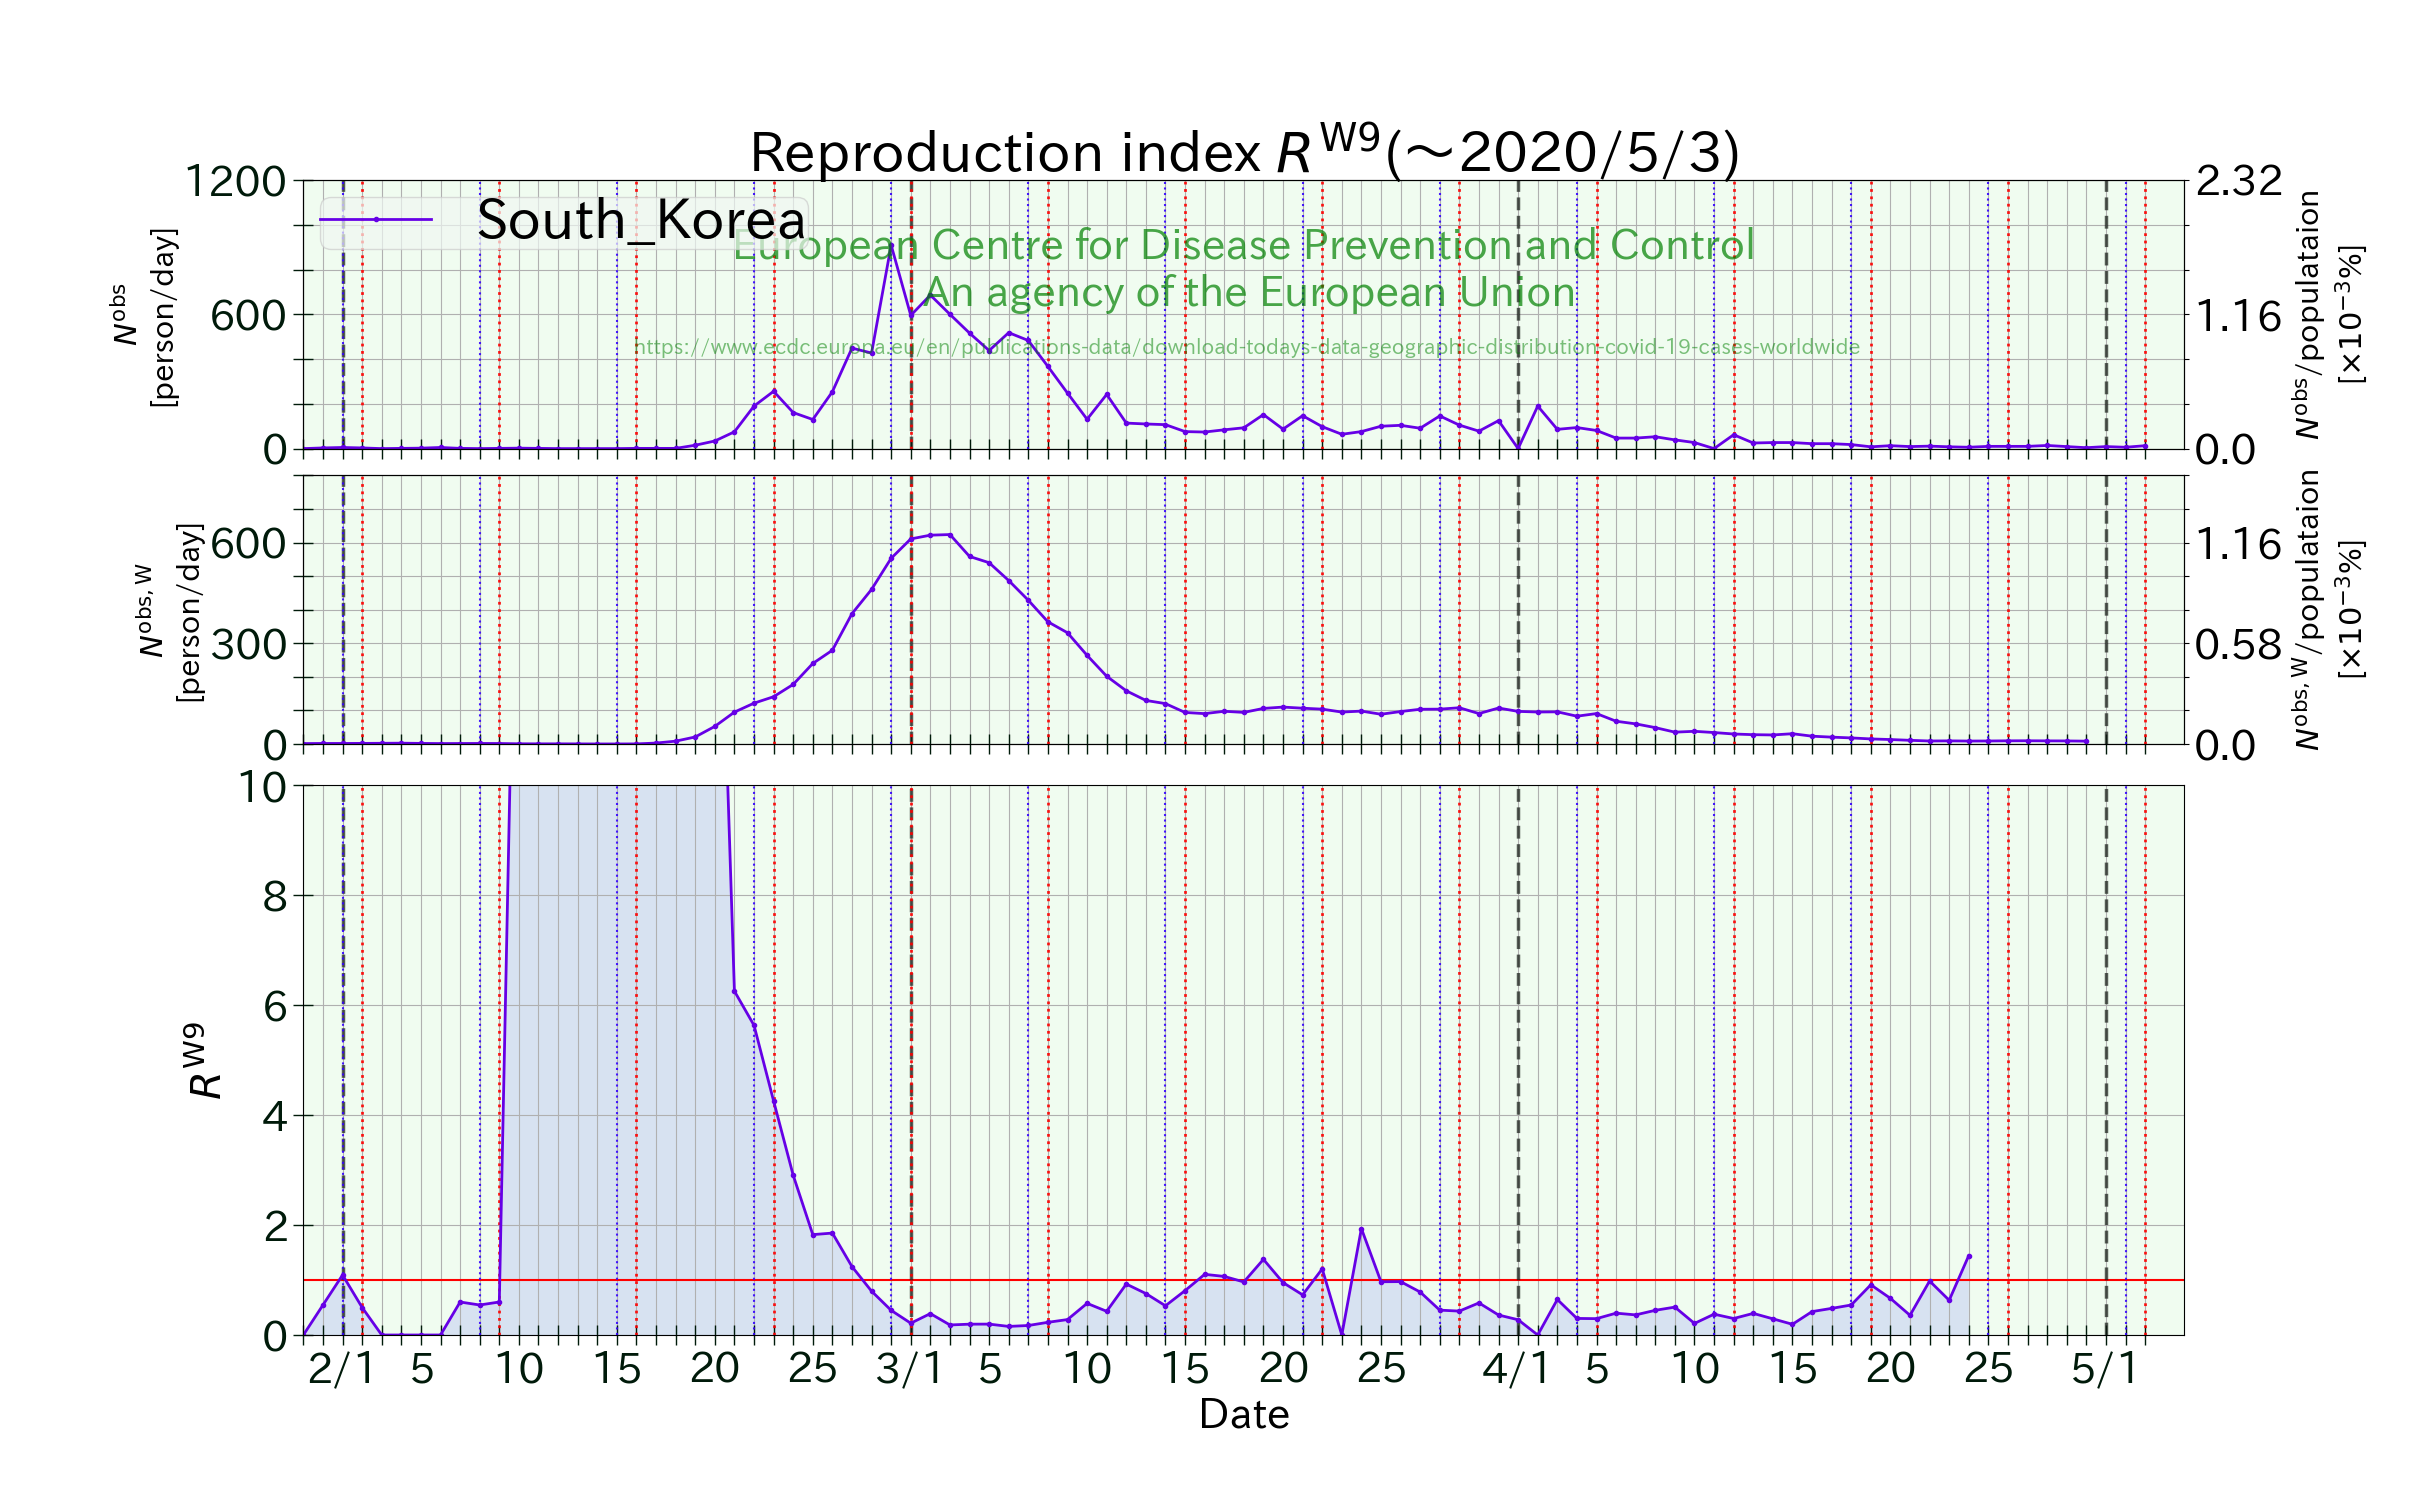
\includegraphics[width=8.9cm]{South_Korea.png}
 \caption{same as fig.1}
 \end{figure*}

\begin{figure*}[ht]
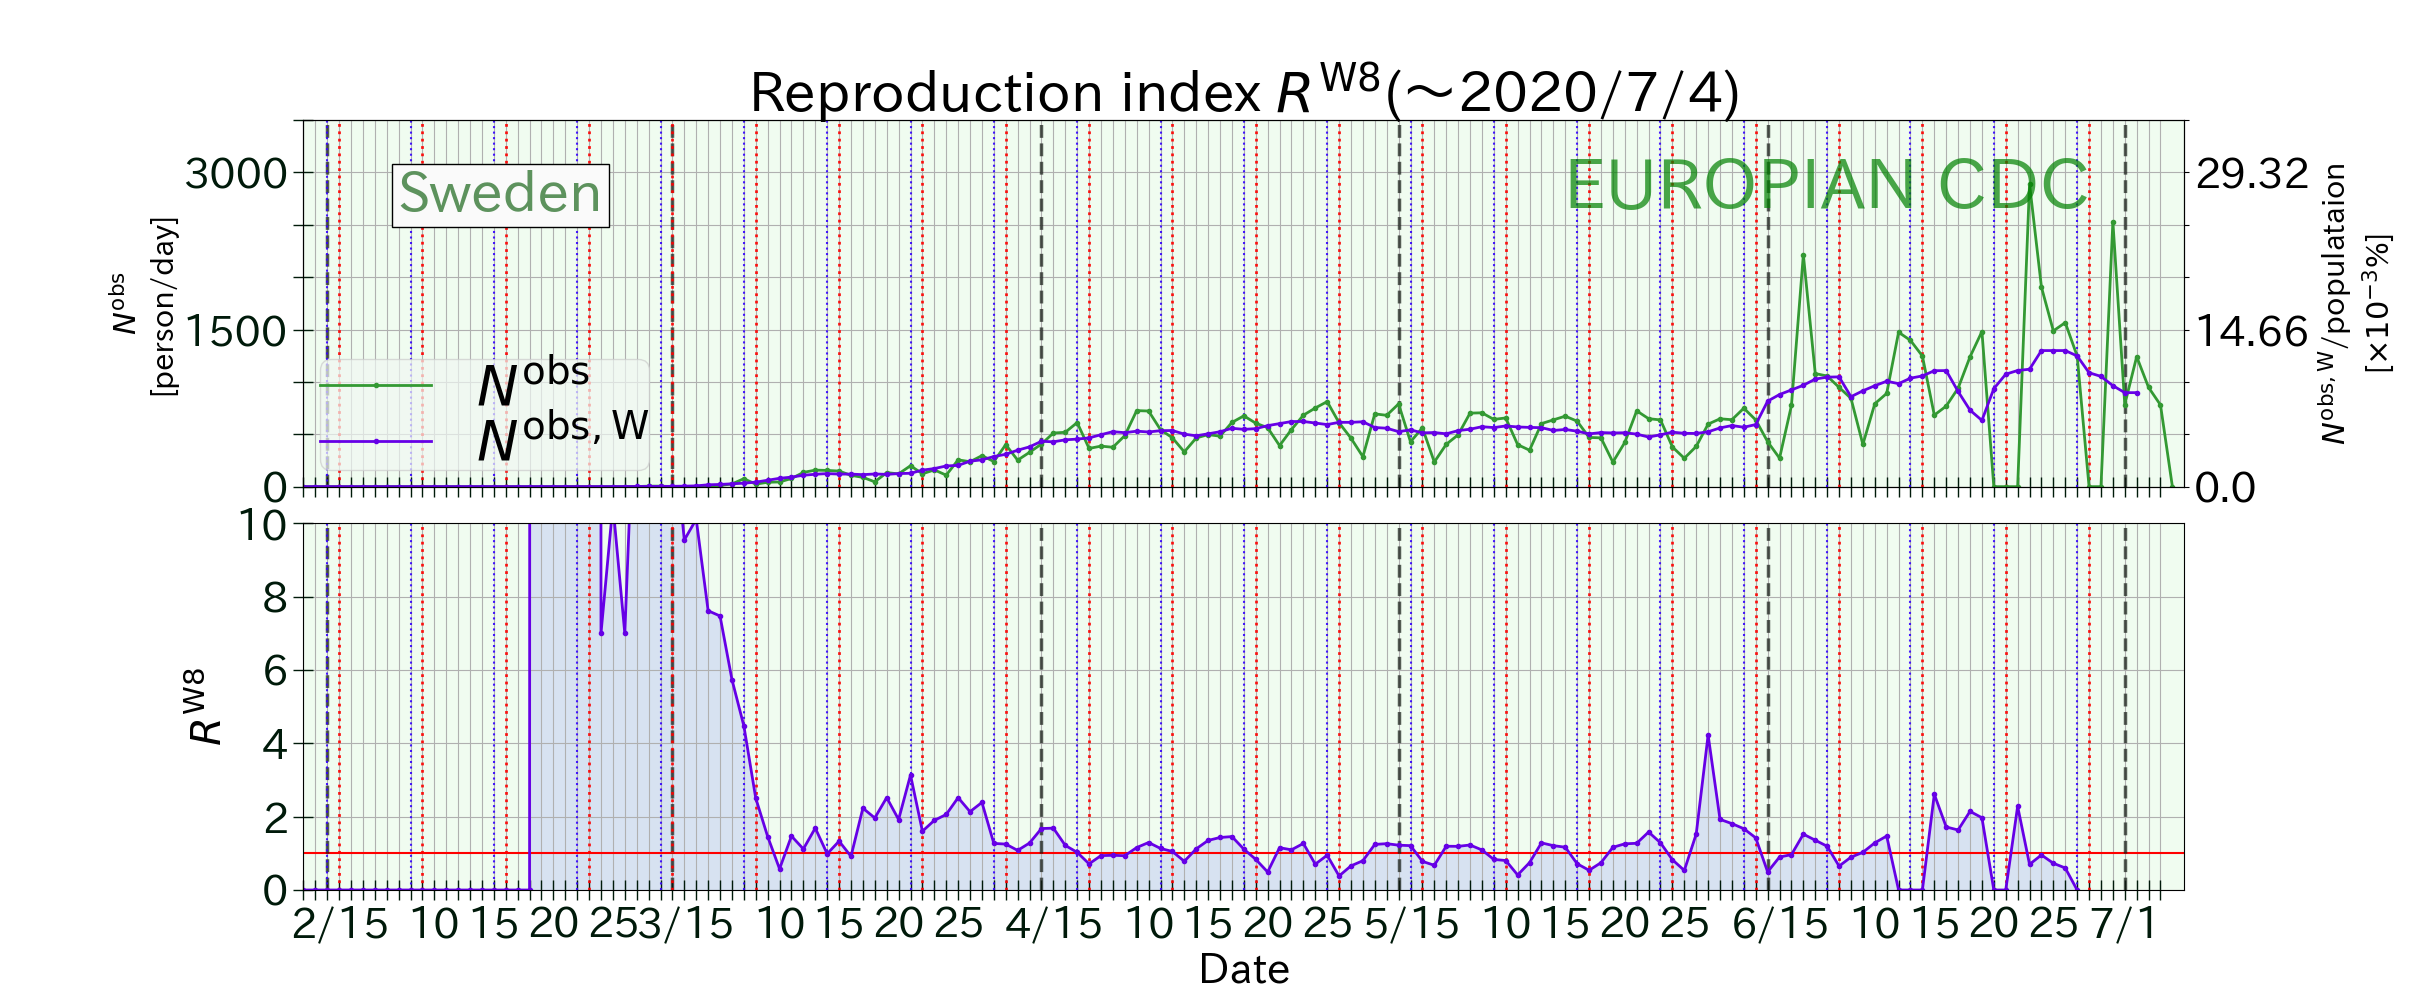
\includegraphics[width=8.9cm]{Sweden.png}
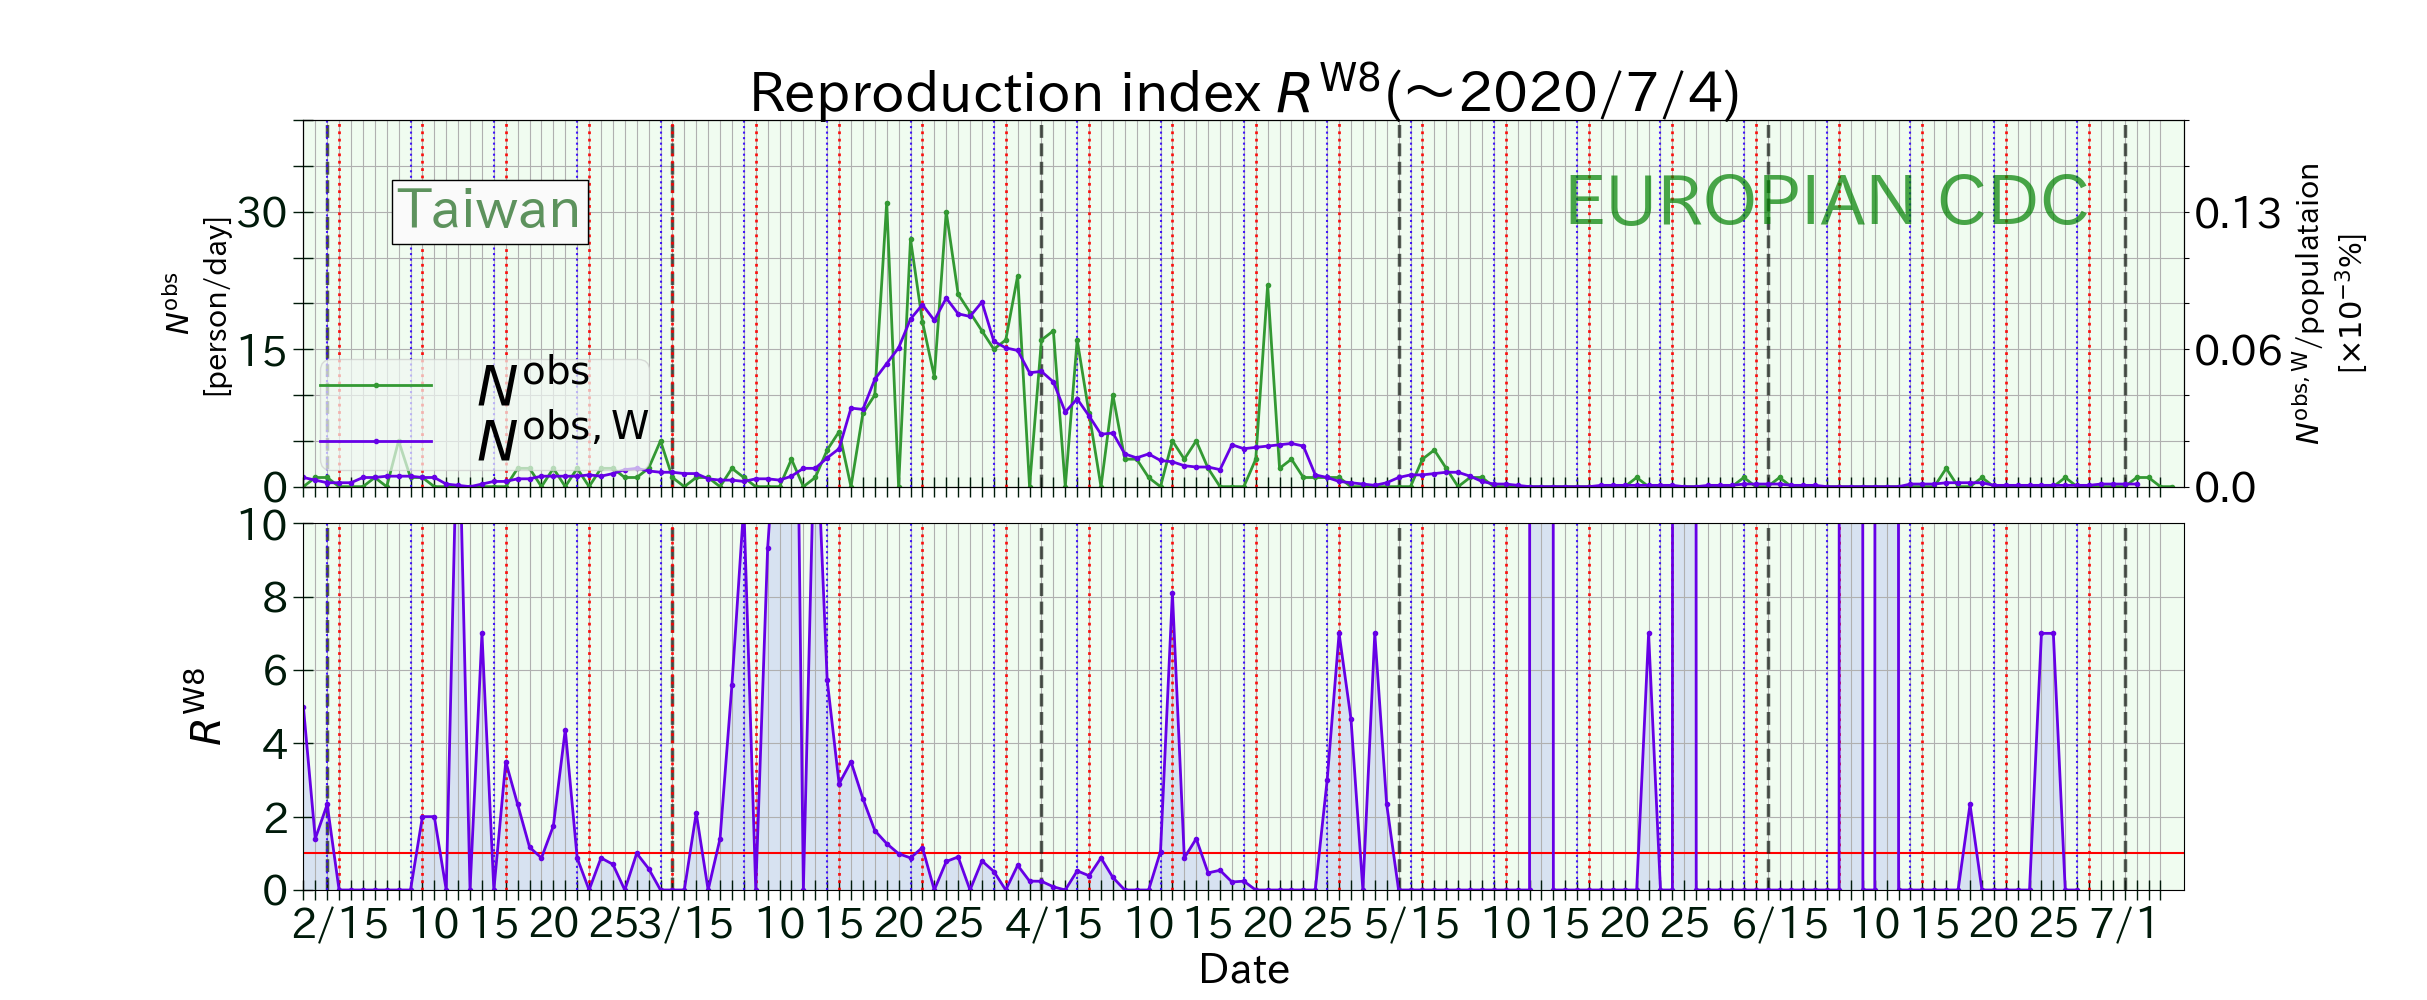
\includegraphics[width=8.9cm]{Taiwan.png}
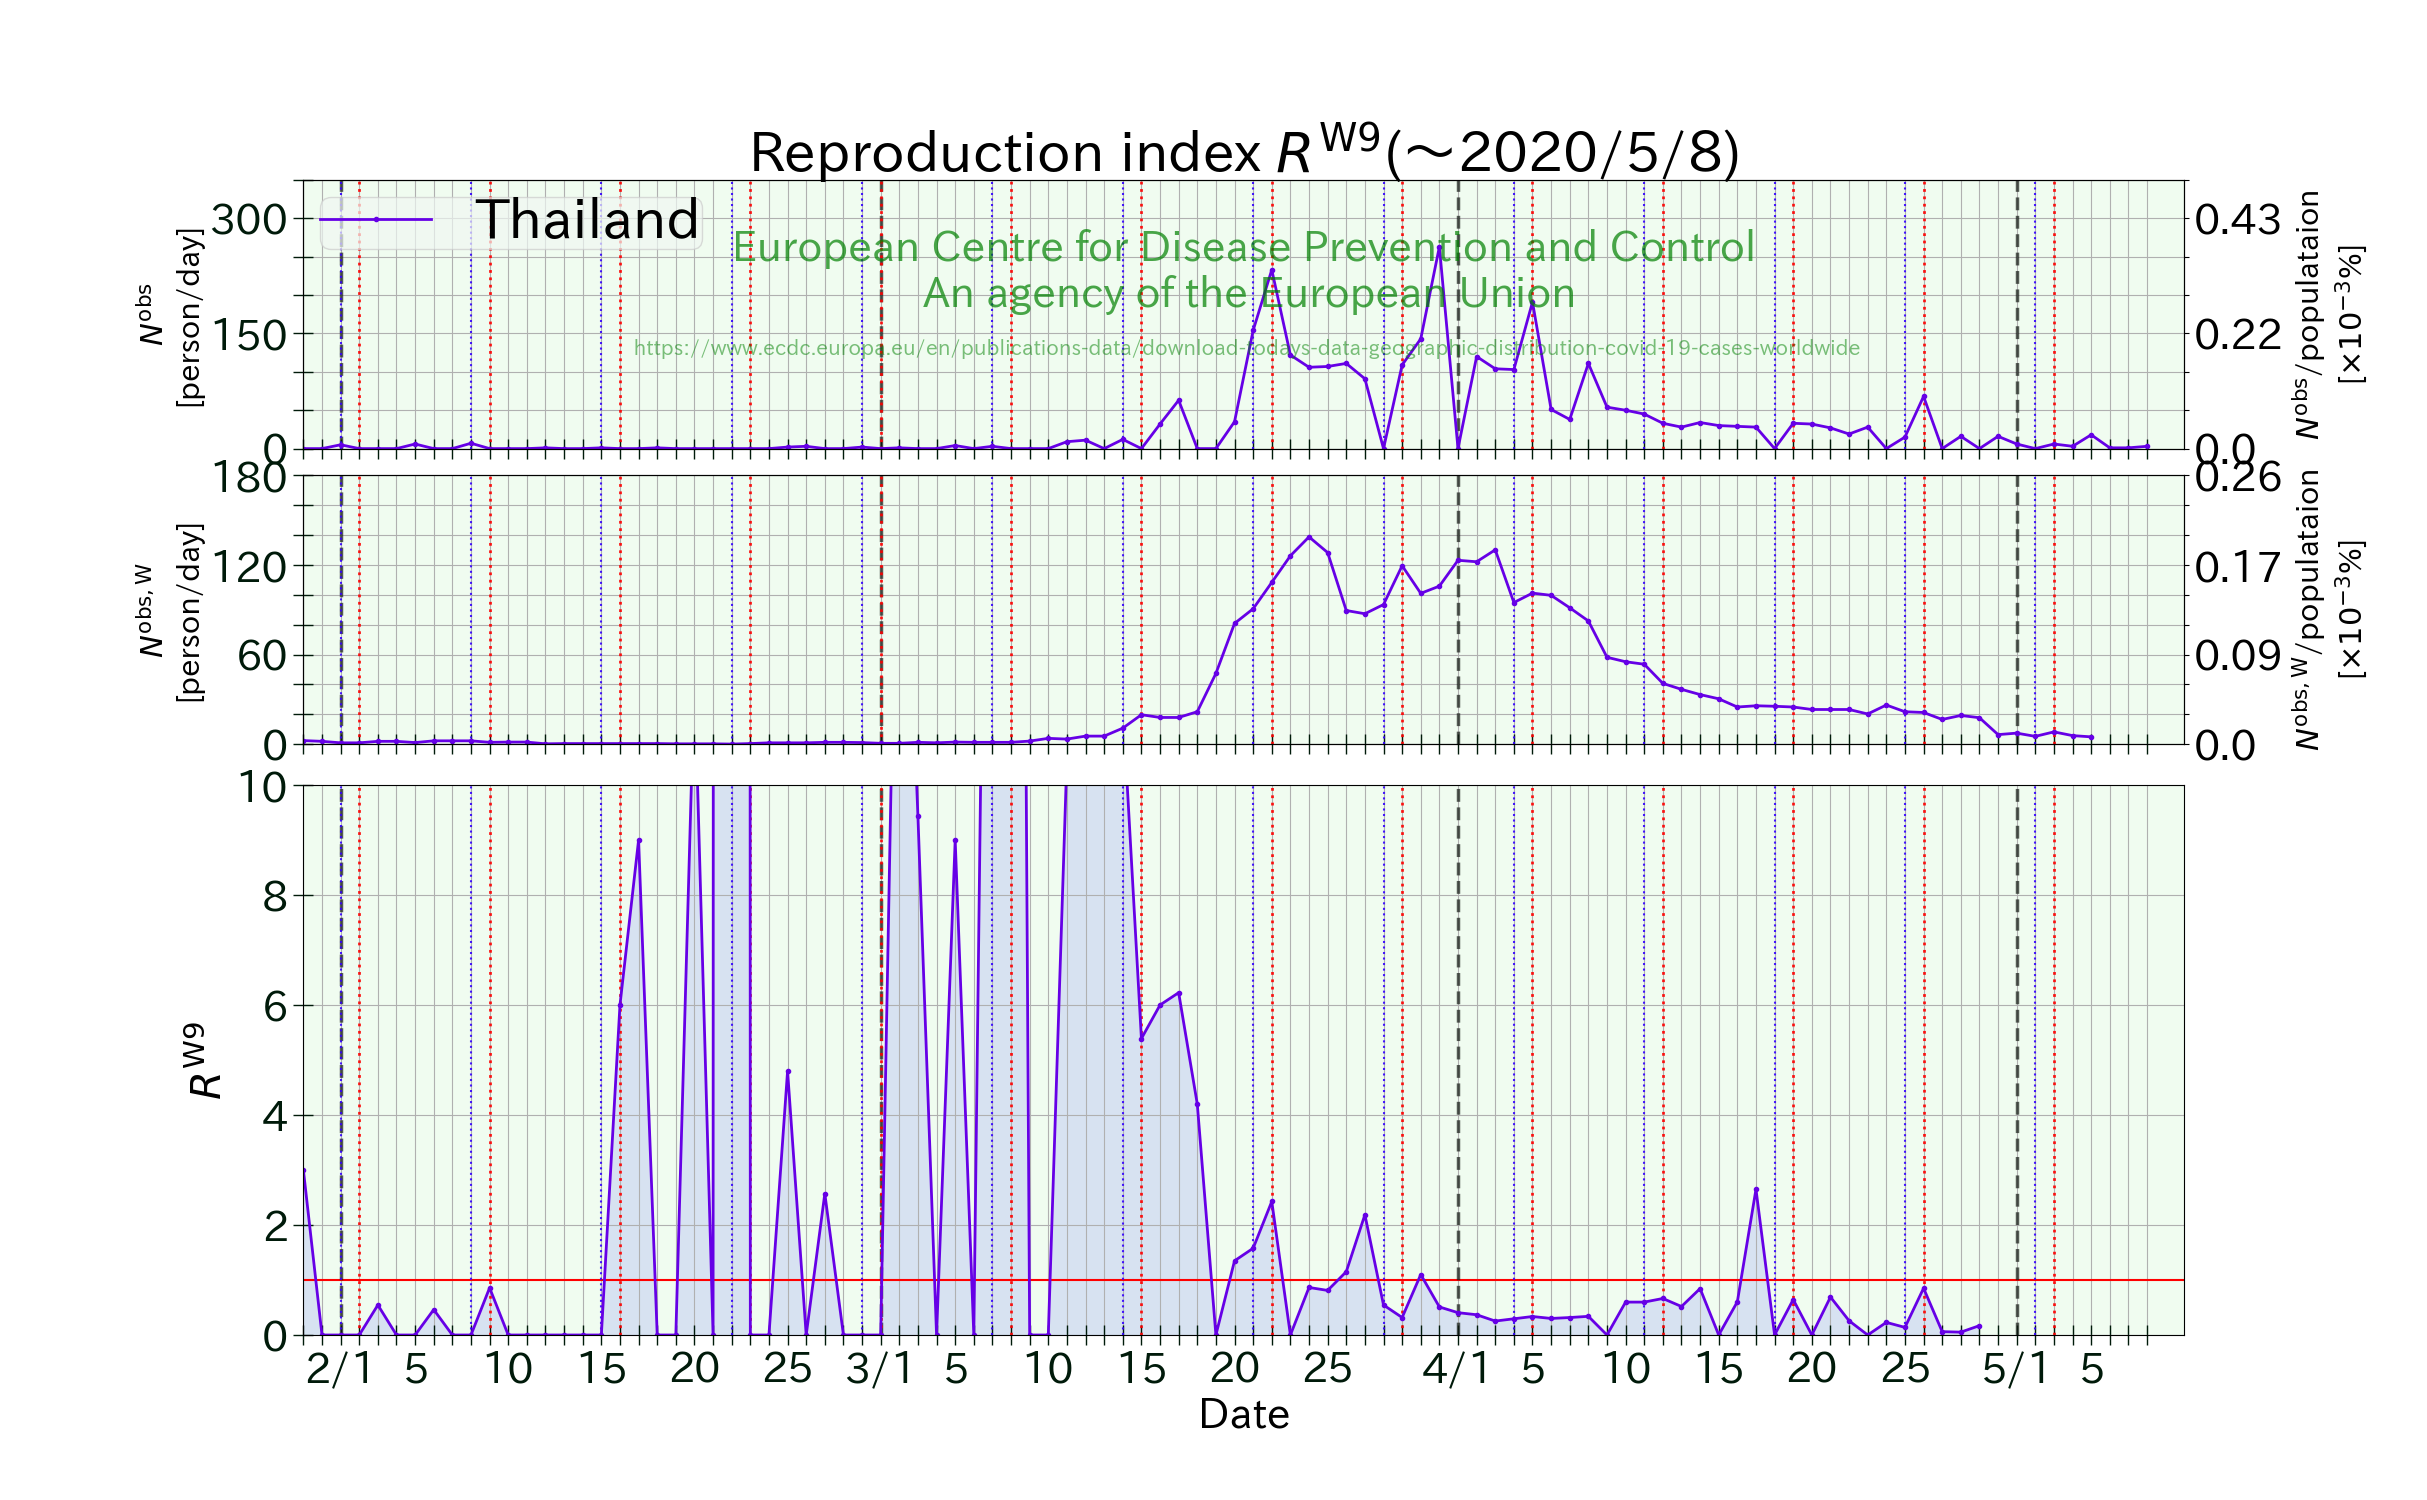
\includegraphics[width=8.9cm]{Thailand.png}
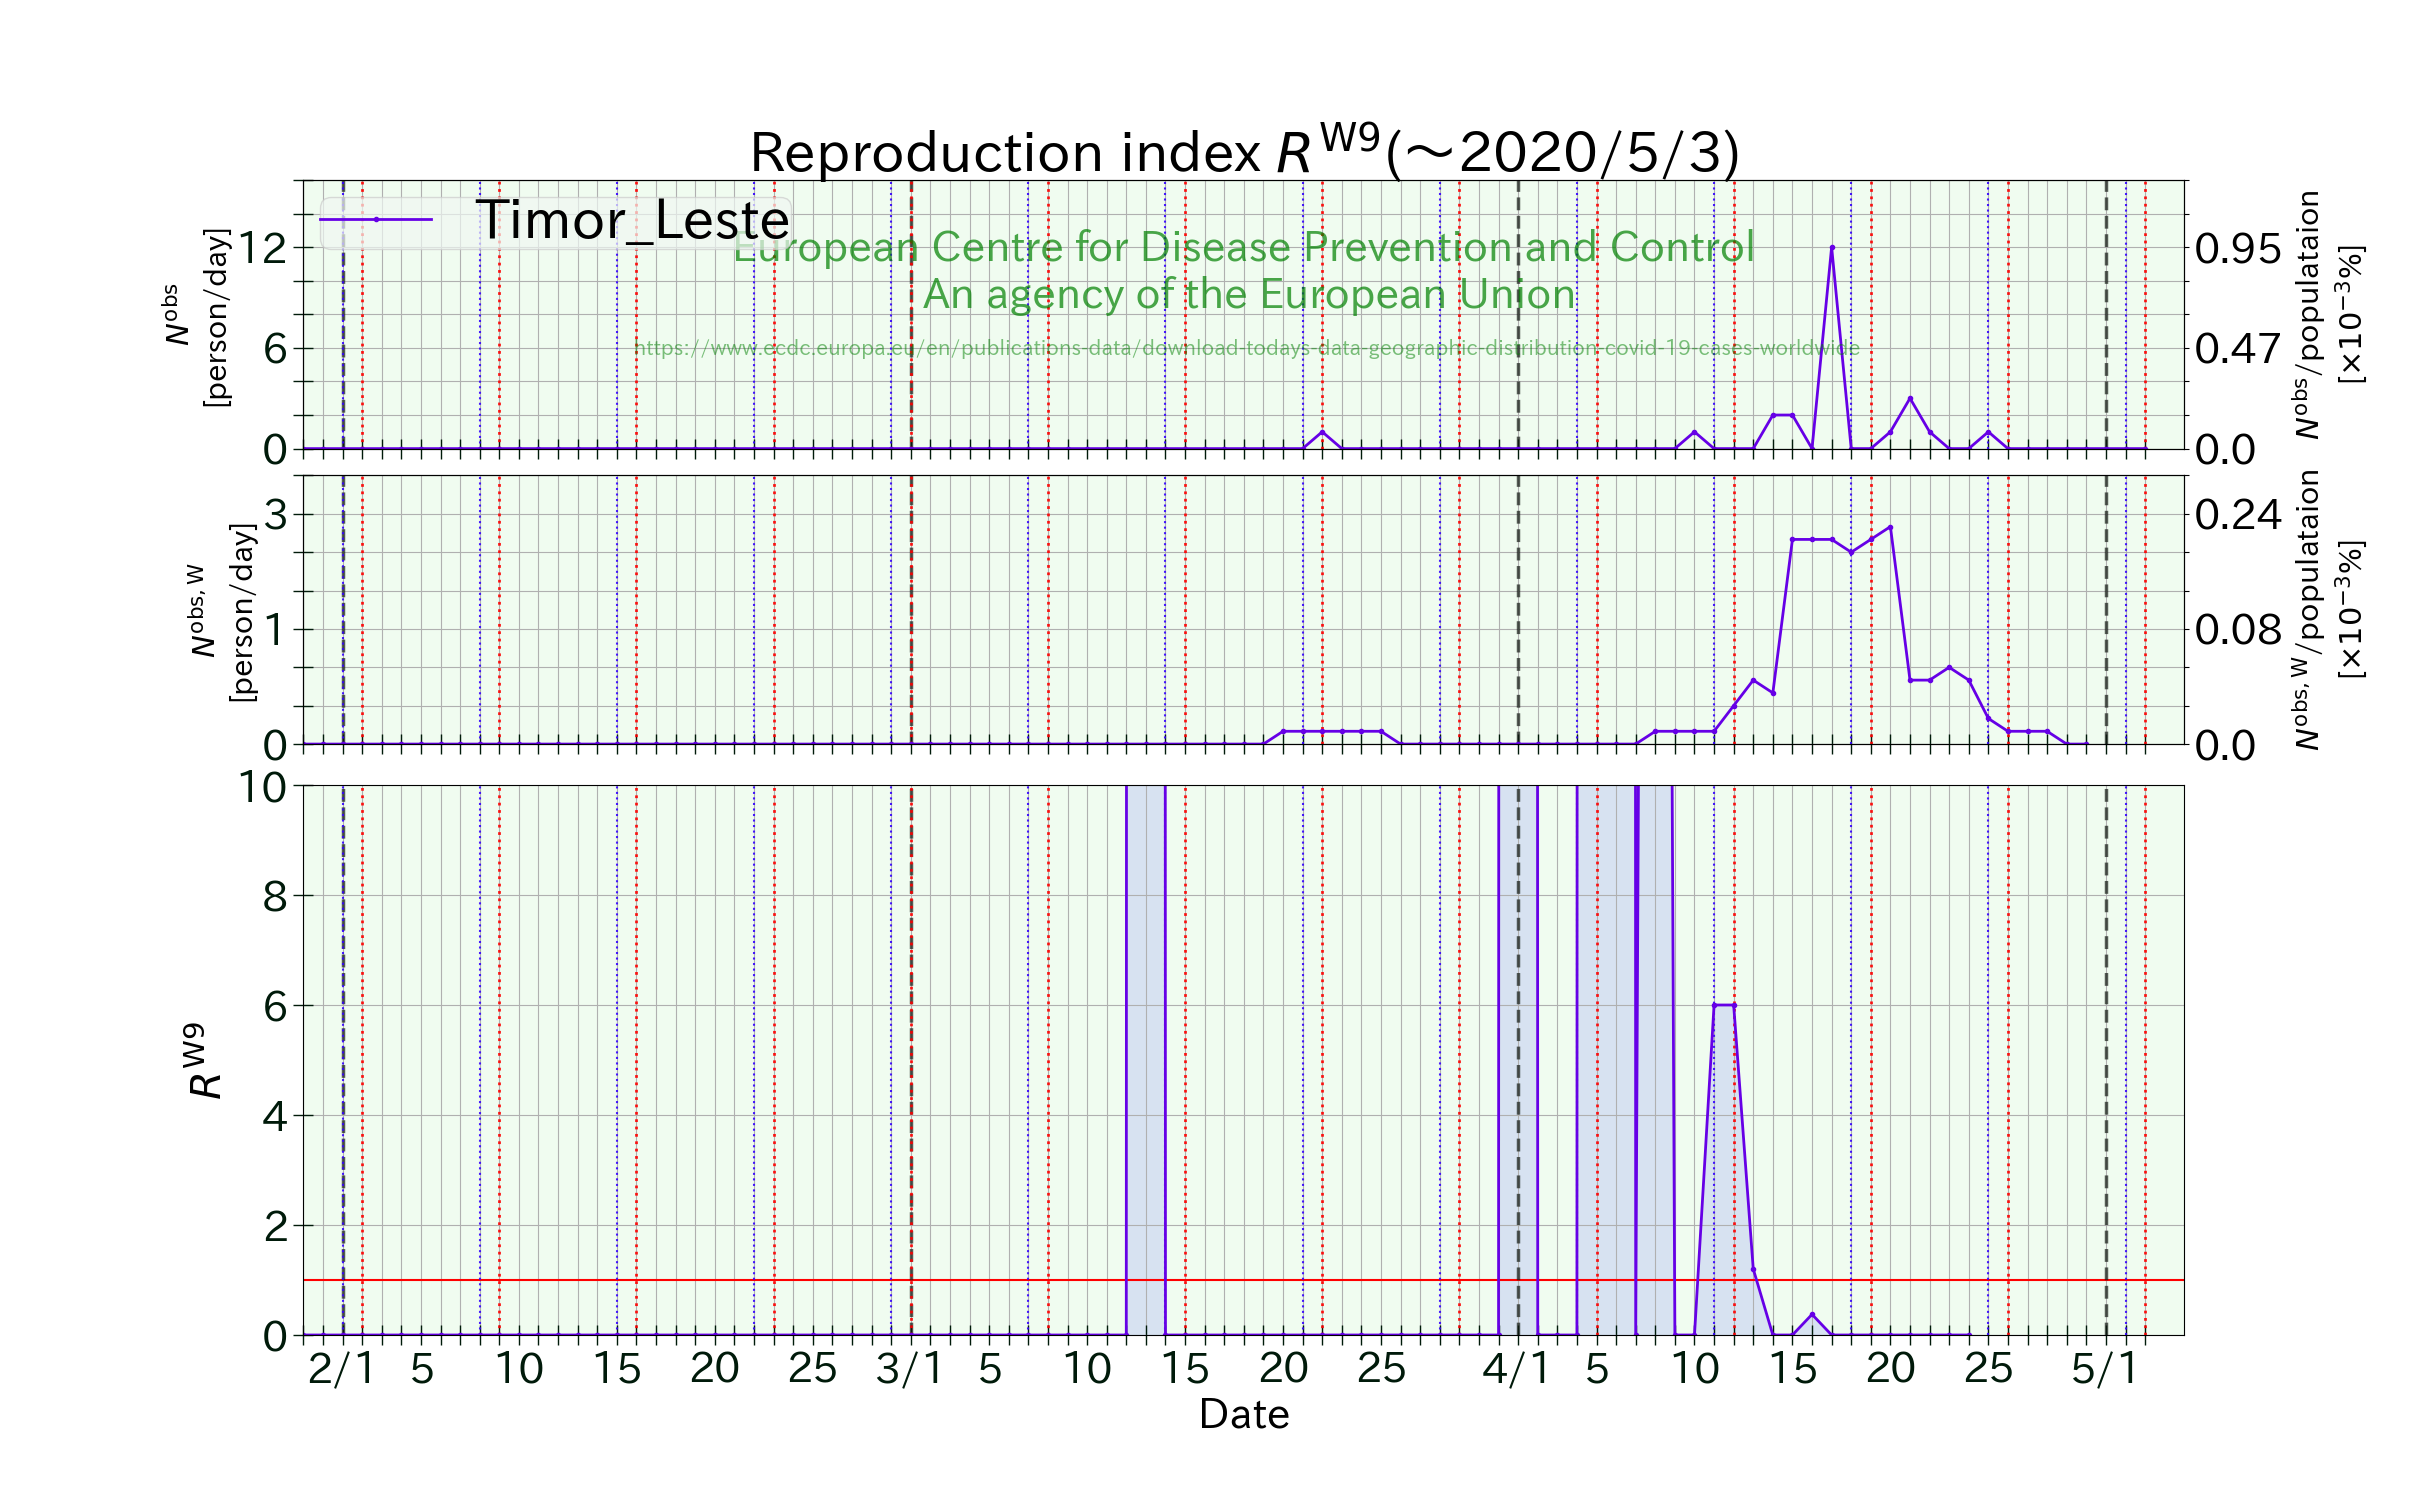
\includegraphics[width=8.9cm]{Timor_Leste.png}
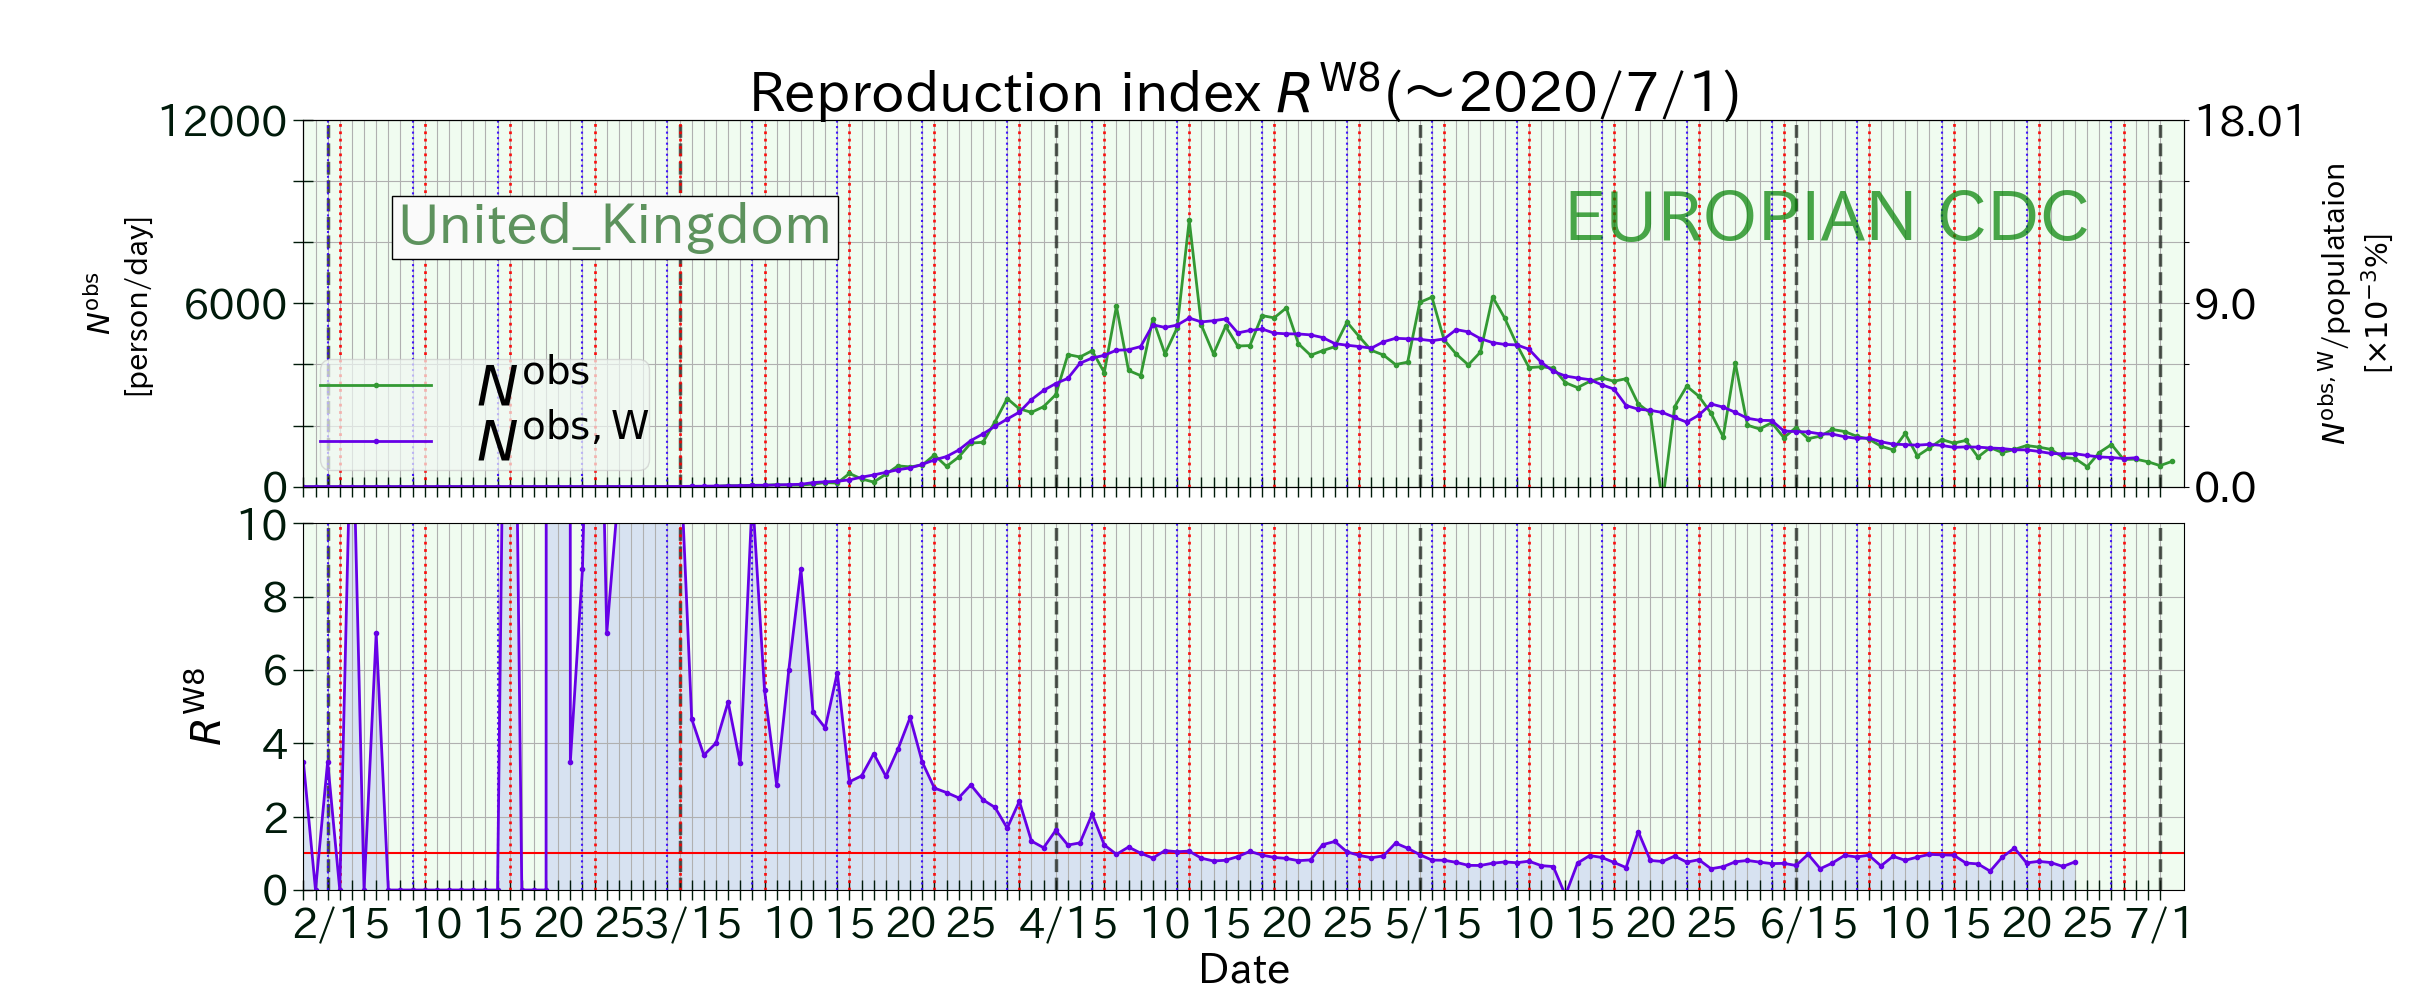
\includegraphics[width=8.9cm]{United_Kingdom.png}
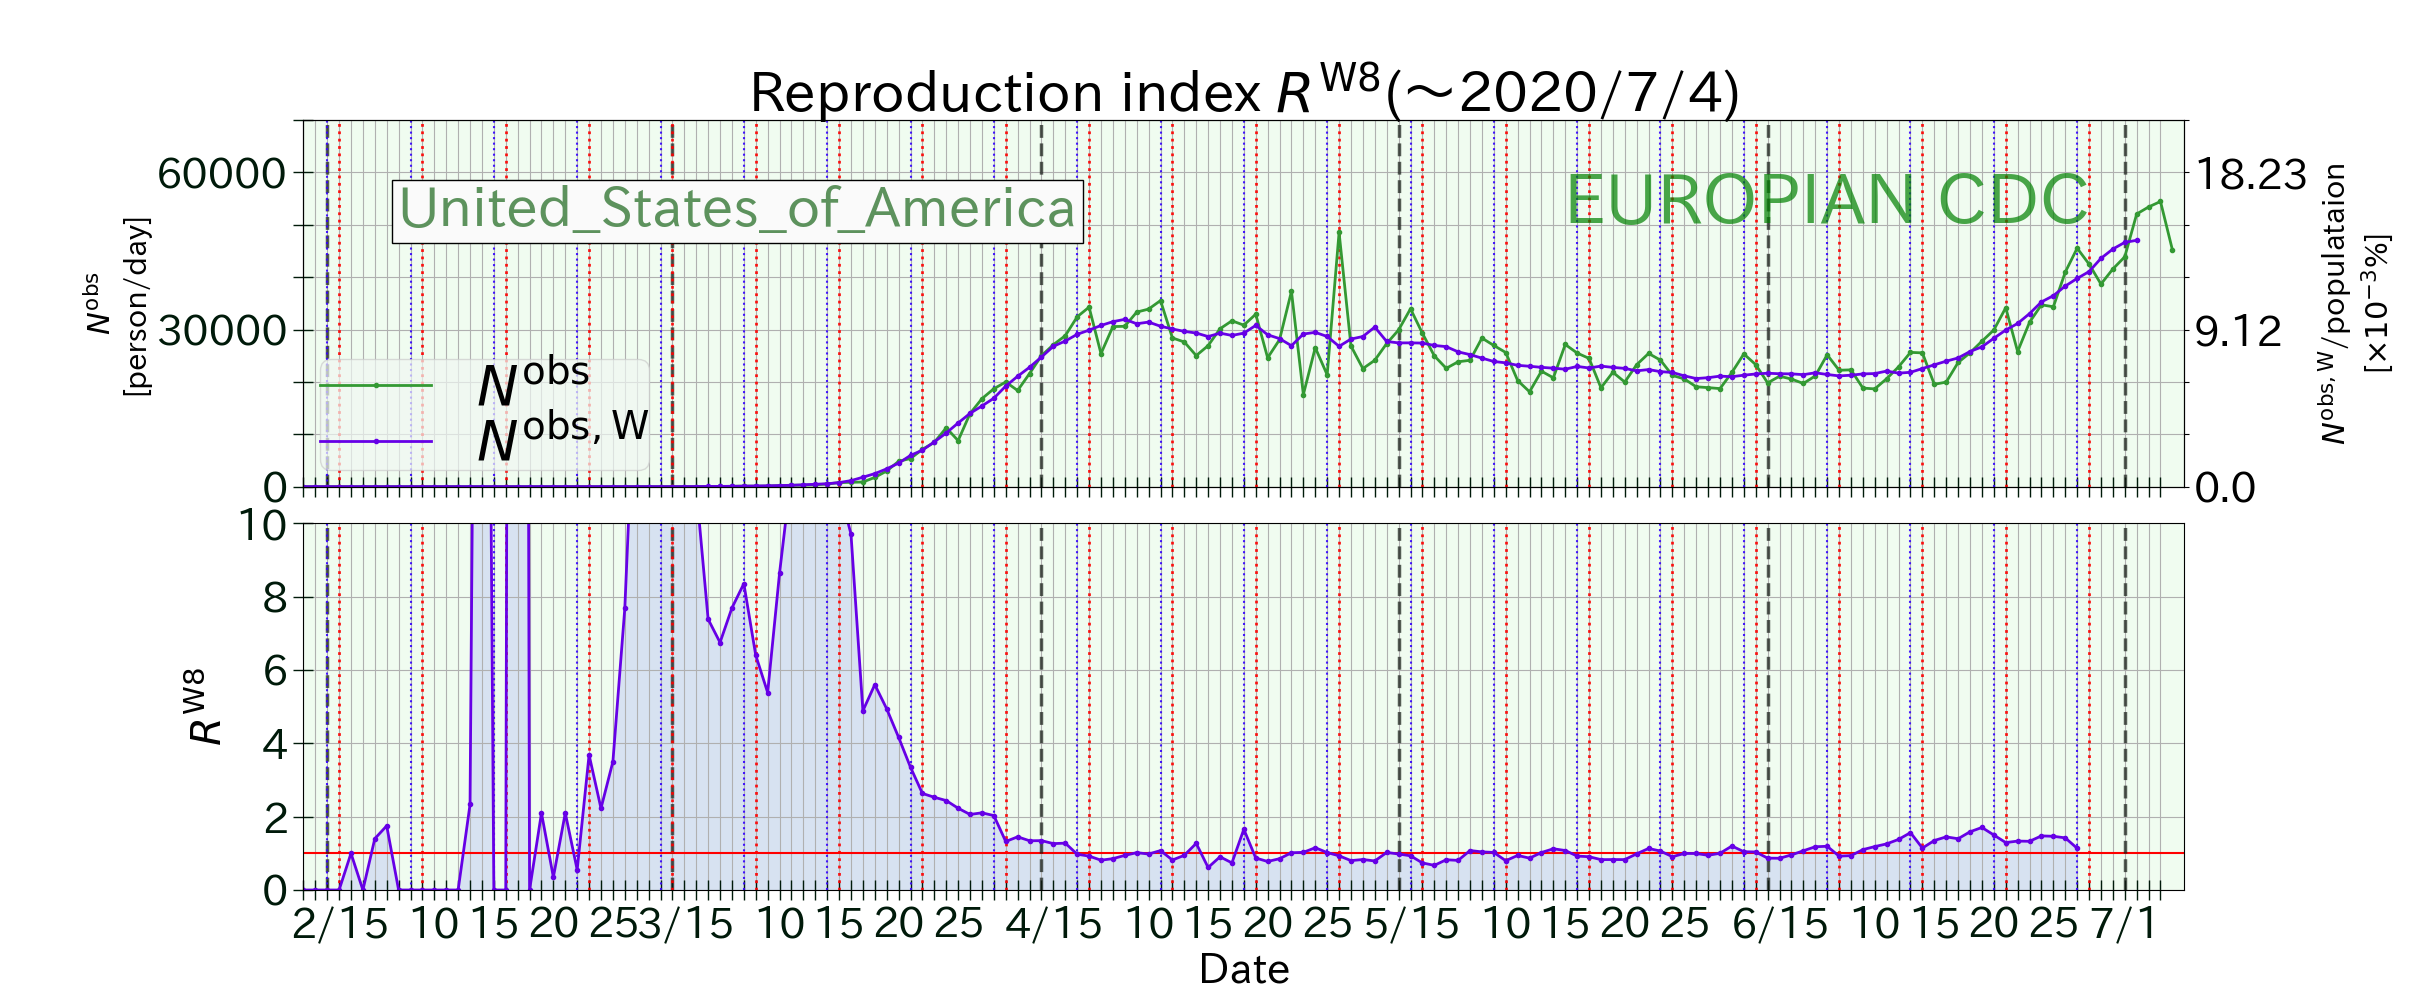
\includegraphics[width=8.9cm]{United_States_of_America.png}
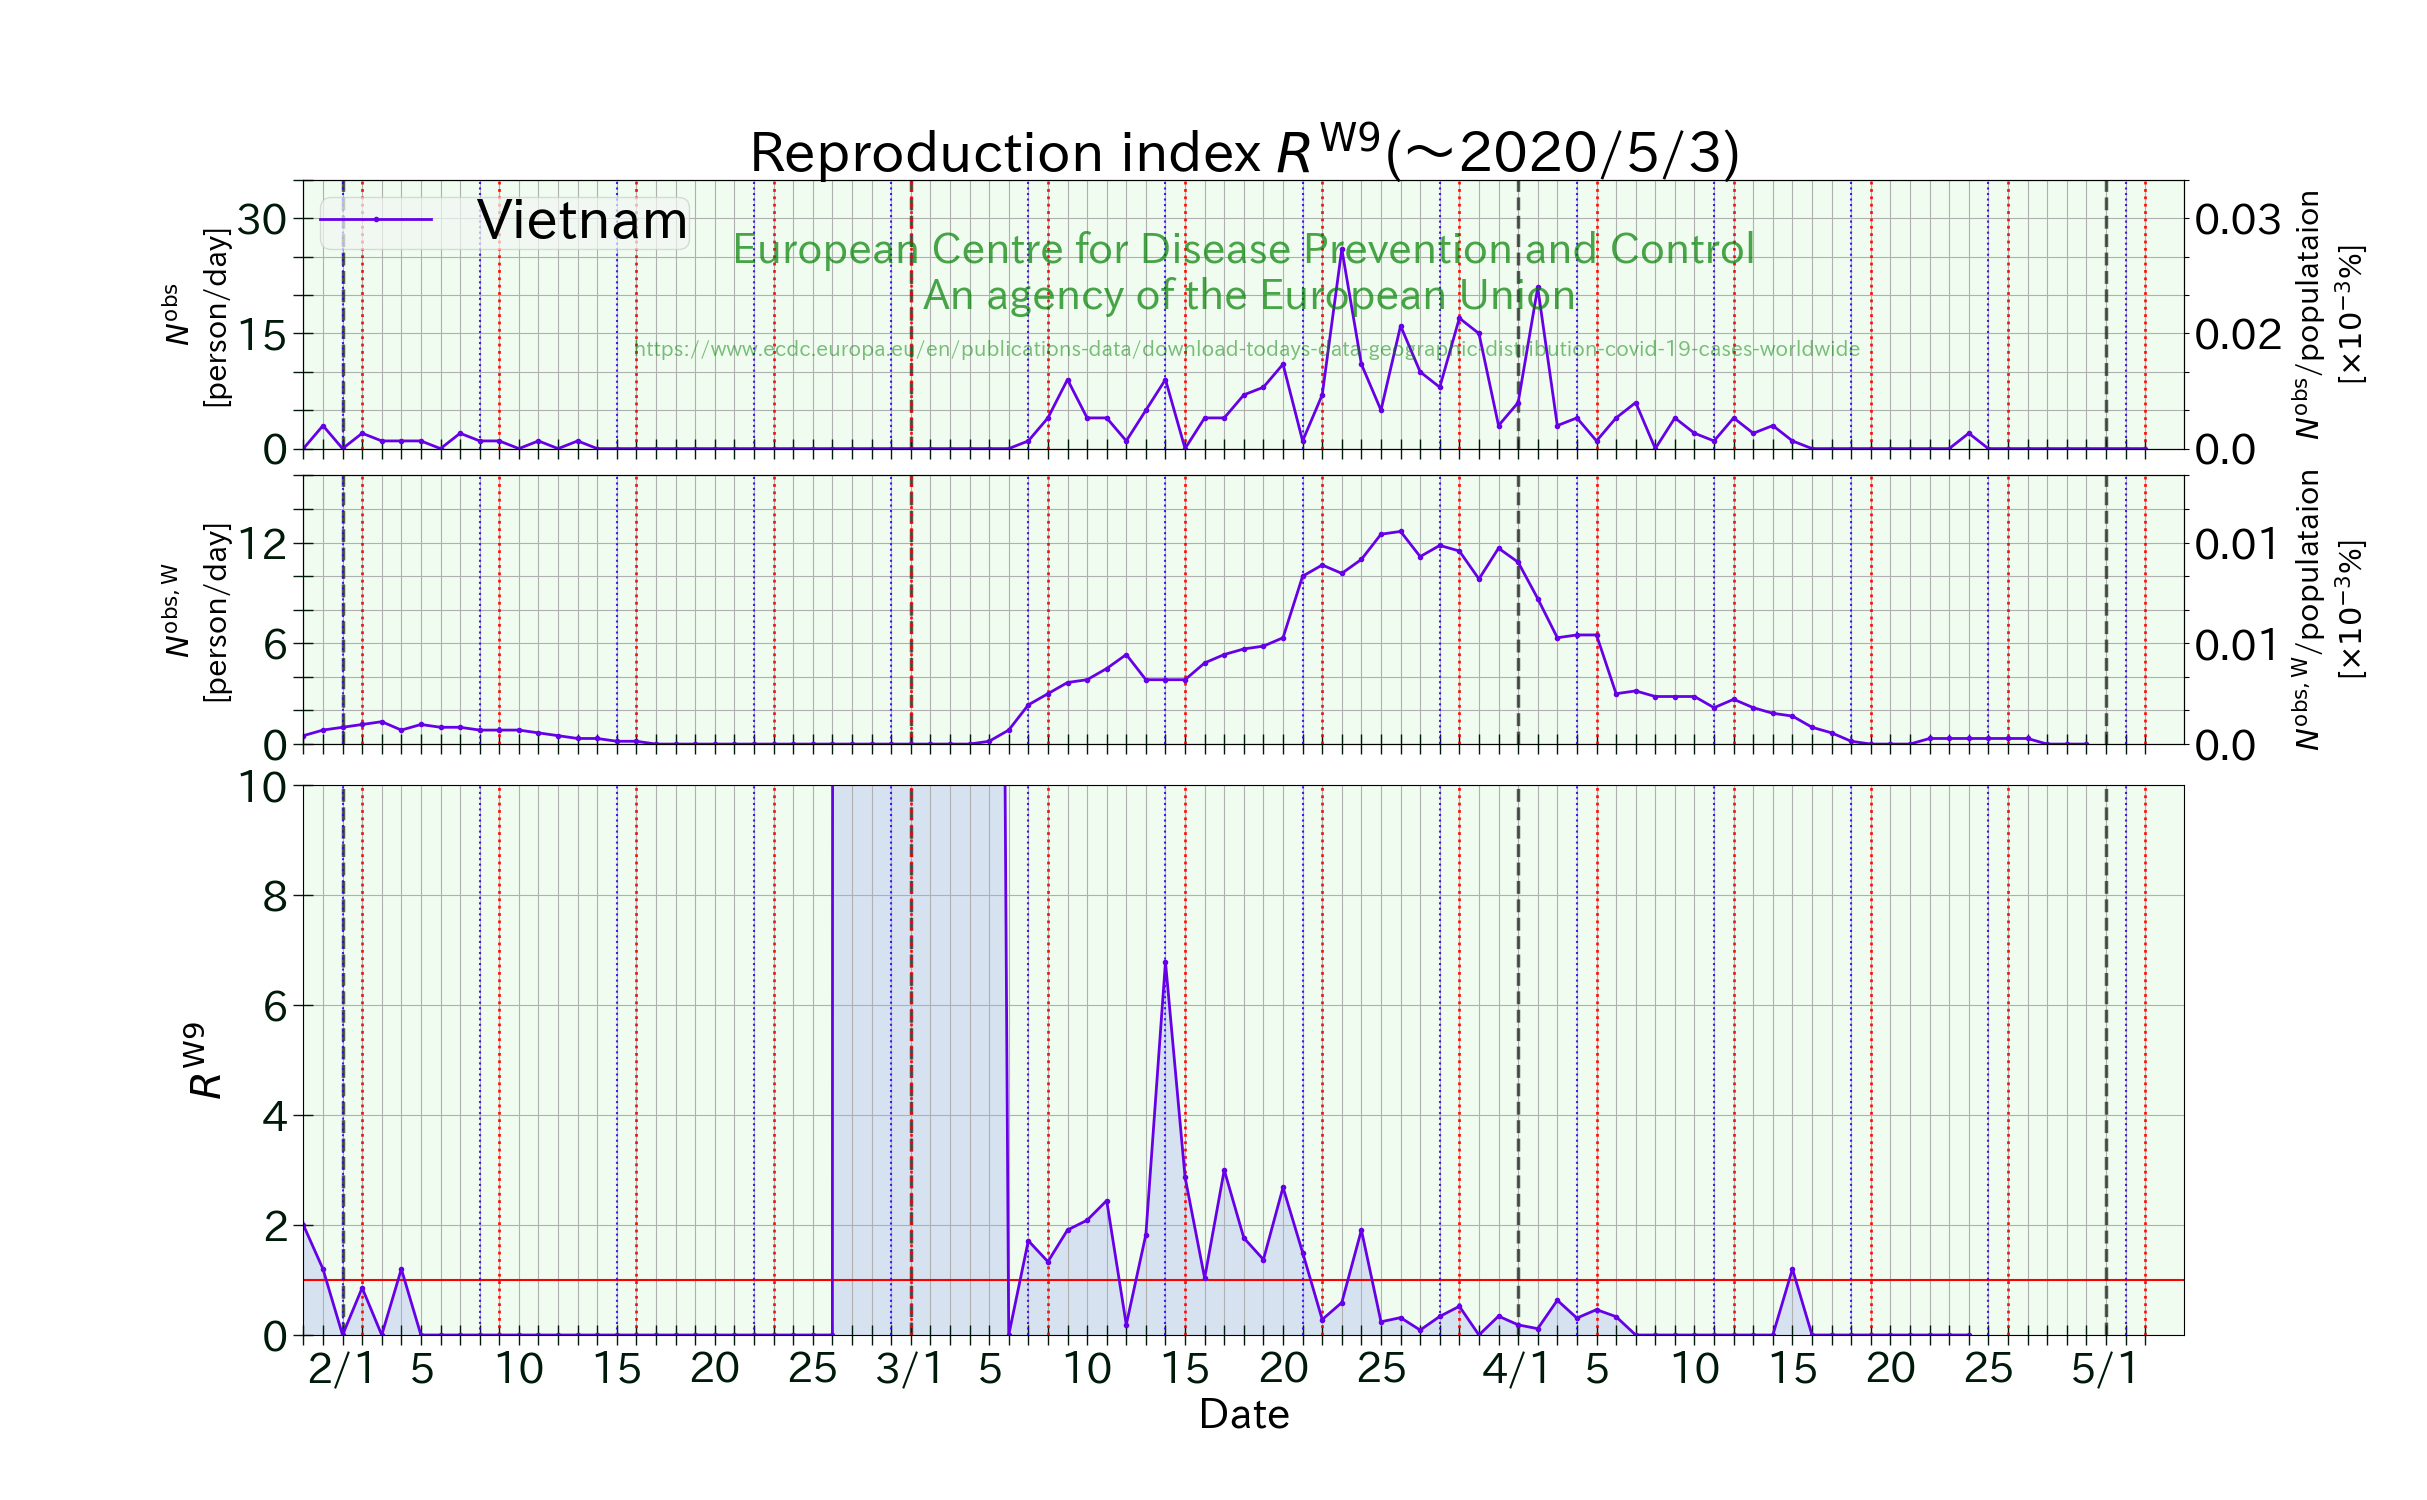
\includegraphics[width=8.9cm]{Vietnam.png}
 \caption{same as fig.1}
 \end{figure*}

\end{document}

